\documentclass[a4paper,11pt,fleqn,twoside,openright,oldfontcommand]{memoir} 	% Openright aabner kapitler paa hoejresider (openany begge)

%%%% PAKKER %%%%

% ¤¤ Oversaettelse og tegnsaetning ¤¤ %
\usepackage[utf8]{inputenc}					% Input-indkodning af tegnsaet (UTF8)
\usepackage[danish]{babel}					% Dokumentets sprog
\usepackage[T1]{fontenc}					% Output-indkodning af tegnsaet (T1)
\usepackage{ragged2e,anyfontsize}			% Justering af elementer
\usepackage{fixltx2e}						% Retter forskellige fejl i LaTeX-kernen
			
																
% ¤¤ Figurer og tabeller (floats) ¤¤ %
\usepackage{graphicx} 						% Haandtering af eksterne billeder (JPG, PNG, PDF)
\usepackage{multirow}                		% Fletning af raekker og kolonner (\multicolumn og \multirow)
\usepackage{colortbl} 						% Farver i tabeller (fx \columncolor, \rowcolor og \cellcolor)
\usepackage[dvipsnames]{xcolor}				% Definer farver med \definecolor. Se mere: http://en.wikibooks.org/wiki/LaTeX/Colors
\usepackage{flafter}						% Soerger for at floats ikke optraeder i teksten foer deres reference
\let\newfloat\relax 						% Justering mellem float-pakken og memoir
\usepackage{float}							% Muliggoer eksakt placering af floats, f.eks. \begin{figure}[H]
%\usepackage{eso-pic}						% Tilfoej billedekommandoer paa hver side
%\usepackage{wrapfig}						% Indsaettelse af figurer omsvoebt af tekst. \begin{wrapfigure}{Placering}{Stoerrelse}
%\usepackage{multicol}         	        	% Muliggoer tekst i spalter
%\usepackage{rotating}						% Rotation af tekst med \begin{sideways}...\end{sideways}

% ¤¤ Matematik mm. ¤¤
\usepackage{amsmath,amssymb,stmaryrd} 		% Avancerede matematik-udvidelser
\usepackage{mathtools}						% Andre matematik- og tegnudvidelser
\usepackage{textcomp}                 		% Symbol-udvidelser (f.eks. promille-tegn med \textperthousand )
\usepackage{siunitx}						% Flot og konsistent praesentation af tal og enheder med \si{enhed} og \SI{tal}{enhed}
\sisetup{output-decimal-marker = {,}}		% Opsaetning af \SI (DE for komma som decimalseparator) 
\usepackage[version=3]{mhchem} 				% Kemi-pakke til flot og let notation af formler, f.eks. \ce{Fe2O3}
%\usepackage{rsphrase}						% Kemi-pakke til RS-saetninger, f.eks. \rsphrase{R1}

% ¤¤ Referencer og kilder ¤¤ %
\usepackage[danish]{varioref}				% Muliggoer bl.a. krydshenvisninger med sidetal (\vref)
\usepackage[numbers,sort&compress]{natbib}

% ¤¤ Misc. ¤¤ %
\usepackage{listings}						% Placer kildekode i dokumentet med \begin{lstlisting}...\end{lstlisting}
\usepackage{lipsum}							% Dummy text \lipsum[..]
\usepackage[shortlabels]{enumitem}			% Muliggoer enkelt konfiguration af lister
\usepackage{pdfpages}						% Goer det muligt at inkludere pdf-dokumenter med kommandoen \includepdf[pages={x-y}]{fil.pdf}	
\pdfoptionpdfminorversion=6					% Muliggoer inkludering af pdf dokumenter, af version 1.6 og hoejere
\pretolerance=2500 							% Justering af afstand mellem ord (hoejt tal, mindre orddeling og mere luft mellem ord)
\usepackage{geometry}
\usepackage{titlesec}  						%needs recent version of »titlesec«
\usepackage{xcolor}

% Kommentarer og rettelser med \fxnote. Med 'final' i stedet for 'draft' udloeser hver note en error i den faerdige rapport.
\usepackage[footnote,draft,danish,silent,nomargin]{fixme}		


%%%% BRUGERDEFINEREDE INDSTILLINGER %%%%

% ¤¤ Marginer ¤¤ %
\setlrmarginsandblock{3.0cm}{3.0cm}{*}		% \setlrmarginsandblock{Indbinding}{Kant}{Ratio}
\setulmarginsandblock{3.0cm}{3.0cm}{*}		% \setulmarginsandblock{Top}{Bund}{Ratio}
\checkandfixthelayout 						% Oversaetter vaerdier til brug for andre pakker

%	¤¤ Afsnitsformatering ¤¤ %
\setlength{\parindent}{0mm}           		% Stoerrelse af indryk
\setlength{\parskip}{3mm}          			% Afstand mellem afsnit ved brug af double Enter
\linespread{1,1}							% Linie afstand

% ¤¤ Litteraturlisten ¤¤ %
\bibliographystyle{unsrtnat}

% ¤¤ Indholdsfortegnelse ¤¤ %
\setsecnumdepth{subsection}		 			% Dybden af nummerede overkrifter (part/chapter/section/subsection)
\maxsecnumdepth{subsection}					% Dokumentklassens graense for nummereringsdybde
\settocdepth{subsection} 					% Dybden af indholdsfortegnelsen

% ¤¤ Lister ¤¤ %
\setlist{
  topsep=0pt,								% Vertikal afstand mellem tekst og listen
  itemsep=-1ex,								% Vertikal afstand mellem items
} 

% ¤¤ Visuelle referencer ¤¤ %
\usepackage[colorlinks]{hyperref}			% Danner klikbare referencer (hyperlinks) i dokumentet.
\hypersetup{colorlinks = true,				% Opsaetning af farvede hyperlinks (interne links, citeringer og URL)
    linkcolor = black,
    citecolor = black,
    urlcolor = black
}

% ¤¤ Opsaetning af figur- og tabeltekst ¤¤ %
\captionnamefont{\small\bfseries\itshape}	% Opsaetning af tekstdelen ('Figur' eller 'Tabel')
\captiontitlefont{\small}					% Opsaetning af nummerering
\captiondelim{. }							% Seperator mellem nummerering og figurtekst
\hangcaption								% Venstrejusterer flere-liniers figurtekst under hinanden
\captionwidth{\linewidth}					% Bredden af figurteksten
\setlength{\belowcaptionskip}{0pt}			% Afstand under figurteksten
		
% ¤¤ Opsaetning af listings ¤¤ %
\definecolor{commentGreen}{RGB}{34,139,24}
\definecolor{stringPurple}{RGB}{208,76,239}

\lstset{language=Matlab,					% Sprog
	basicstyle=\ttfamily\scriptsize,		% Opsaetning af teksten
	keywords={for,if,while,else,elseif,		% Noegleord at fremhaeve
			  end,break,return,case,
			  switch,function},
	keywordstyle=\color{blue},				% Opsaetning af noegleord
	commentstyle=\color{commentGreen},		% Opsaetning af kommentarer
	stringstyle=\color{stringPurple},		% Opsaetning af strenge
	showstringspaces=false,					% Mellemrum i strenge enten vist eller blanke
	numbers=left, numberstyle=\tiny,		% Linjenumre
	extendedchars=true, 					% Tillader specielle karakterer
	columns=flexible,						% Kolonnejustering
	breaklines, breakatwhitespace=true,		% Bryd lange linjer
}

% ¤¤ Navngivning ¤¤ %
\addto\captionsdanish{
	\renewcommand\appendixname{Bilag}
	\renewcommand\contentsname{Indholdsfortegnelse}	
	\renewcommand\appendixpagename{Bilag}
	\renewcommand\appendixtocname{Bilag}
	\renewcommand\cftchaptername{\chaptername~}				% Skriver "Kapitel" foran kapitlerne i indholdsfortegnelsen
	\renewcommand\cftappendixname{\appendixname~}			% Skriver "Appendiks" foran appendiks i indholdsfortegnelsen
}

% ¤¤ Kapiteludssende ¤¤ %
\definecolor{numbercolor}{gray}{0.7}		% Definerer en farve til brug til kapiteludseende
\newif\ifchapternonum

\makechapterstyle{jenor}{					% Definerer kapiteludseende frem til ...
  \renewcommand\beforechapskip{0pt}
  \renewcommand\printchaptername{}
  \renewcommand\printchapternum{}
  \renewcommand\printchapternonum{\chapternonumtrue}
  \renewcommand\chaptitlefont{\fontfamily{pbk}\fontseries{db}\fontshape{n}\fontsize{25}{35}\selectfont\raggedleft}
  \renewcommand\chapnumfont{\fontfamily{pbk}\fontseries{m}\fontshape{n}\fontsize{1in}{0in}\selectfont\color{numbercolor}}
  \renewcommand\printchaptertitle[1]{%
    \noindent
    \ifchapternonum
    \begin{tabularx}{\textwidth}{X}
    {\let\\\newline\chaptitlefont ##1\par} 
    \end{tabularx}
    \par\vskip-2.5mm\hrule
    \else
    \begin{tabularx}{\textwidth}{Xl}
    {\parbox[b]{\linewidth}{\chaptitlefont ##1}} & \raisebox{-15pt}{\chapnumfont \thechapter}
    \end{tabularx}
    \par\vskip2mm\hrule
    \fi
  }
}											% ... her

\chapterstyle{jenor}						% Valg af kapiteludseende - Google 'memoir chapter styles' for alternativer

% ¤¤ Sidehoved/sidefod ¤¤ %

\makepagestyle{Uni}							% Definerer sidehoved og sidefod udseende frem til ...
\makepsmarks{Uni}{%
	\createmark{chapter}{left}{shownumber}{}{. \ }
	\createmark{section}{right}{shownumber}{}{. \ }
	\createplainmark{toc}{both}{\contentsname}
	\createplainmark{lof}{both}{\listfigurename}
	\createplainmark{lot}{both}{\listtablename}
	\createplainmark{bib}{both}{\bibname}
	\createplainmark{index}{both}{\indexname}
	\createplainmark{glossary}{both}{\glossaryname}
}
\nouppercaseheads											% Ingen Caps oenskes

\makeevenhead{Uni}{Gruppe c2-15a}{}{\leftmark}				% Lige siders sidehoved (\makeevenhead{Navn}{Venstre}{Center}{Hoejre})
\makeoddhead{Uni}{\rightmark}{}{Aalborg Universitet}			% Ulige siders sidehoved (\makeoddhead{Navn}{Venstre}{Center}{Hoejre})
\makeevenfoot{Uni}{\thepage}{}{}							% Lige siders sidefod (\makeevenfoot{Navn}{Venstre}{Center}{Hoejre})
\makeoddfoot{Uni}{}{}{\thepage}								% Ulige siders sidefod (\makeoddfoot{Navn}{Venstre}{Center}{Hoejre})
\makeheadrule{Uni}{\textwidth}{0.5pt}						% Tilfoejer en streg under sidehovedets indhold
\makefootrule{Uni}{\textwidth}{0.5pt}{1mm}					% Tilfoejer en streg under sidefodens indhold

\copypagestyle{Unichap}{Uni}								% Sidehoved defineres som blank på kapitelsider
\makeoddhead{Unichap}{}{}{}
\makeevenhead{Unichap}{}{}{}
\makeheadrule{Unichap}{\textwidth}{0pt}
\aliaspagestyle{chapter}{Unichap}							% Den ny style vaelges til at gaelde for chapters
															% ... her
															
\pagestyle{Uni}												% Valg af sidehoved og sidefod (benyt "plain" for ingen sidehoved/fod)


%%%% EGNE KOMMANDOER %%%%

% ¤¤ Billede hack ¤¤ %										% Indsaet figurer nemt med \figur{Stoerrelse}{Fil}{Figurtekst}{Label}
\newcommand{\figur}[4]{
		\begin{figure}[H] \centering
			\includegraphics[width=#1\textwidth]{billeder/#2}
			\caption{#3}
			\label{#4}
		\end{figure} 
}

% ¤¤ Specielle tegn ¤¤ %
\newcommand{\decC}{^{\circ}\text{C}}
\newcommand{\dec}{^{\circ}}
\newcommand{\m}{\cdot}


%%%% ORDDELING %%%%

\hyphenation{In-te-res-se e-le-ment}

%%%% MACRO %%%%

\newenvironment{folderinput}[1]{%
\let\finput\input
\renewcommand{\input}[1]{\finput{#1/##1}}}%
{\let\input\finput}


%% ^^Alt setup findes i preamble^^ %%
\raggedbottom

\begin{document}
\frontmatter %% romertegn som sidetal %%

%% folderinput er så man frit kan flytte filerne ned til de relevante mapper %%

	\begin{folderinput}{Setup}
Hello World!
\cleardoublepage
% Dette er LaTeX-versionen af titelbladet for TNB studenterrapporter
% Filen kræver:
% Universitetets logo:  AAU-logo-stud-UK eller AAU-logo-stud-DK
% Synopsis: En fil ved navn synopsis.tex

% Udarbejdet af: Jesper Nørgaard (jesper@noergaard.eu) 10. april 2012
% Redigeret af Mathias S. Hansen (mat_elm13@hotmial.com) 9. november 2016

%\phantomsection
\thispagestyle{empty}
%\pdfbookmark[0]{Titelblad}{titelblad}

\begin{minipage}[t]{0.48\textwidth}
\vspace*{-25pt}			%\vspace*{-9pt}

\includegraphics[height=4cm]{billeder/AAU-logo-stud-DK-RGB}
\end{minipage}
\hfill
\begin{minipage}[t]{0.48\textwidth}
{\small 
\textbf{Første Studieår v/ }\\
\textbf{School of Engineering and Science (SES)}  \\
Energi \\
Strandvejen 12-14 \\
9000 Aalborg \\
http://www.tnb.aau.dk}
\end{minipage}

\vspace*{0.2cm}

\begin{minipage}[t]{0.48\textwidth}
\textbf{Titel:} \\[5pt]\bigskip\hspace{2ex}
Trådløs Mobilopladning

\textbf{Projekt:} \\[5pt]\bigskip\hspace{2ex}
P1

\textbf{Projektperiode:} \\[5pt]\bigskip\hspace{2ex}
Oktober 2016 - December 2016

\textbf{Projektgruppe:} \\[5pt]\bigskip\hspace{2ex}
C2-16a	

\textbf{Deltagere:} \\[5pt]\hspace*{2ex}

\noindent\begin{tabular}{ll}
\makebox[2.5in]{\hrulefill} \\
Daniel Revsbech Pedersen \\
\end{tabular} \\[10pt]\hspace*{2ex}


\noindent\begin{tabular}{ll}
\makebox[2.5in]{\hrulefill} \\
Mads Lindstrøm Paulsen \\
\end{tabular} \\[10pt]\hspace*{2ex}

\noindent\begin{tabular}{ll}
\makebox[2.5in]{\hrulefill} \\
Mathias Stenberg Hansen \\
\end{tabular} \\[10pt]\hspace*{2ex}

\noindent\begin{tabular}{ll}
\makebox[2.5in]{\hrulefill} \\
Nicolai Nørgaard Munk \\
\end{tabular} \\[10pt]\hspace*{2ex}

\noindent\begin{tabular}{ll}
\makebox[2.5in]{\hrulefill} \\
Sisse Sorgenfri Jensen \\
\end{tabular} \\[10pt]\hspace*{2ex}

\noindent\begin{tabular}{ll}
\makebox[2.5in]{\hrulefill} \\
Torben Brund Jørgensen \\
\end{tabular} \\[10pt]\hspace*{2ex}

%Daniel Revsbech Pedersen \\[5pt]\\\hspace*{2ex}
%Julian Bo Larsen \\[5pt]\\\hspace*{2ex}
%Mads Lindstrøm Paulsen \\[5pt]\\\hspace*{2ex}
%Mathias Stenberg Hansen \\[5pt]\\\hspace*{2ex}
%Nicolai Nørgaard Munk \\[5pt]\\\hspace*{2ex}
%Sisse Sorgenfri Jensen \\[5pt]\\\bigskip\hspace{2ex}
%Torben Brund Jørgensen

\textbf{Vejledere:} \\[10pt]\hspace*{2ex}

\noindent\begin{tabular}{ll}
\makebox[2.5in]{\hrulefill} \\
Christian Uhrenfeldt \\
\end{tabular}
%Christian Uhrenfeldt \\\hspace{2ex}%\\\bigskip\hspace{2ex}

%\vspace*{1cm}

\end{minipage}
\hfill
\begin{minipage}[t]{0.483\textwidth}
Synopsis: \\[5pt]
\fbox{\parbox{7cm}{\bigskipHer kommer vores synopsis til at være.

(TESTER)
Strøm er noget, alle kender til. Det bliver brugt overalt, da næsten alle vores apparater benytter strøm i dag. Samfundet er derfor meget afhængig af at kunne sende strømmen ud til forbrugerne. Dette foregår via et ledningsnetværk, hvor ledningerne enten kan være kabler, som er kravet i jorden, eller så kan det være luftledninger, som er ophængt i master. "(Kilde Gyldendal)" Luftledninger og kabler i jorden er den bedste teknologi, som findes til at sende elektricitet ud til forbrugerene, det er her Wireless Power Transfer (WPT), altså trådløs energioverførelse, kunne være en rigtig god teknologi. Ved at benytte WPT så bliver samfundet fri for at lægge jordkabler eller ophænge luftledninger, men i stedet overføre energien igennem luften og hen til produktet kun ved hjælp af en transmitter og en modtager.\bigskip}}

\vspace*{15,3cm}

\textbf{Oplagstal: ?} \\
\textbf{Sidetal: ?} \\
\textbf{Appendiks: ?} \\ 
\textbf{Afsluttet: 19/12/16}

\end{minipage}

\vfill


%{\footnotesize\itshape Rapportens indhold er frit tilgængeligt, men offentliggørelse (med kildeangivelse) må kun ske efter aftale med forfatterne.}

% Rapportens indhold er frit tilgængeligt, men offentliggørelse (med kildeangivelse) må kun ske efter aftale med forfatterne.
% The content of the report is freely available, but publication (with source reference) may only take place in agreement with the authors.
\cleardoublepage

%% Table of Contents %%
\phantomsection													% Kunstigt afsnit, som hyperlinks kan 'holde fast i'
\pdfbookmark[0]{Indholdsfortegnelse}{indhold}					% Tildeler en klikbar bookmark til den endelige PDF
\tableofcontents*												% Indholdsfortegnelsen (kaldet ToC)

	\end{folderinput}

\mainmatter %% Normale sidetal %%
\chapter{Indledning}
Samfundet vi liver i dag er yderst afhængig af elektricitet for at kunne funger og vi som samfund er blevet var til den afhængighed, hvilke har gennem tiden ført til ny og bedre teknologi, og derved er ideen omkring trådløs energi overførelse også opstået. Trådløs energi overførelse er noget rimeligt nyt, der ses i hverdagen, men teknologien stammer tilbage fra 1890´erne hvor Nikola Tesla havde allerede forsøgte sig med, at skabe og sende trådløs elektricitet, (Bellow,2016) og drømte om at sende energien igennem den øvre atmosfære. Nikola Tesla drømte om fri energi til hele verden ikke blot kun til en by, men der er stadig lang vej den dag i dag. Metoder der bliver brugt i dag har stadig utrolig mange problemstillinger før det vil være muligt og erstatte traditionelle kabler. Før det er muligt, at lade trådløs elektricitet overtage hverdagen, er der nogle krav til denne teknologi 

Der er mange forskellige måder og sende energien på, men et af kravene der er meget vigtige er, at disse metoder ikke gør skade på mennesket, ikke mindst med det er det vigtig at energi kan blive sendt over længere distancer uden for meget spild og ustabil forbindelse. I dag er der meget fokus på global opvarmning og ikke mindst grøn energi, hvor Danmark har 2020 og 2050 planerne derfor er det også vigtigt, at der er tænkt miljøbevist før teknologien ville kunne slå igennem og blive den mest anvendte.

Der er to forskellige tilgange til denne teknologi, WSP (Wireless Power Transfer). En af tilgangene benytter sig af højfrekvens bølger, som mikrobølger eller lasere, en af disse sendes gennem luften hen til en modtager der kan omdanne den modtaget stråle/mikrobølge energien (photonerne) til elektricitet igen. Hvis denne metode anvendes er det muligt, at sende energi over længere afstande uden nogen form for fysik tilkobling, dog er det hovedsaglige problem med denne teknologi, at hvis der kommer noget imellem afsenderen og modtagerne ophøre overførelsen, ikke desto mindre kan det være skadeligt for mennesker, at udsætte dem for strålerne. Den anden tilgangsmåde forholder sig lidt anderledes her anvendes der elektromagnetisme, denne tilgangsmåde benytter sig af de elektroner der løber gennem en ledning, når elektroner løber gennem en ledning skabes der et magnetisk felt omkring (Amperes lov).  Når et magnetisk felt får indflydelse på en ledning skubber det magnetiske felt  til elektronerne, som skaber elektricitet (Faraday´s lov). I sådan et system har i forhold til den anden tilgang en begrænset rækkevidde, men den er alt mere sikker at anvende for mennesker. Denne teknologi bliver i dag brugt til flere forskellige produkter, eksempelvis bliver det brugt til og lade elektriske tandbørster op med og ikke mindst til pacemakers. Dette er denne type teknologi projektet vil fokuser på. 
 %% Står hernede da den rodede rundt i kapitlerne %%

	\begin{folderinput}{Problemanalyse}
\chapter{Problemanalyse}
\section{Introduktion: Trådløs energioverførsel}

Noget der kommer lige efter indledning:

Hvor ser man wpt i dag?

Trådløs energioverførsel eller trådløs opladning er i dag implementeret i forskellige produkter bl.a. mellem en elektrisk tandbørste og dens opladerstation. Til selve energioverførslen benyttes induktiv kobling oftest, da det effektivt er muligt at overføre energien over en kort afstand. Induktiv kobling er en form af elektromagnetisme. Andre typer indenfor elektromagnetisme som mikrobølger kan også benyttes til trådløs energioverførsel, men da mikrobølger har en skadelig effekt på levende organismer, og induktiv kobling allerede bliver benyttet til formålet energioverførsel, så ser vi derved nærmere på denne type af elektromagnetisme.

**(MIT-artikel)** Flere fordele for induktiv kobling...

Hvorfor er det relevant at kigge på wpt i dag?

Man kan altid spørge om, hvor vi ser teknologien i fremtiden, men et andet vigtigt perspektiv er, hvor relevant trådløs energioverførsel er i dag. Vi er et progressivt folkefærd, og vi vil altid gerne anerkendes for vores projekter. Vi er nået så langt, som vi kan nå med ledninger, så det næste skridt må være at fjerne ledningerne. Med den store ændring i regeringernes klimaaftaler, skal vi også tænke på transport. Vi bliver nød til at finde en måde at få vores elbiler til at køre længere, en måde at kunne gøre det kan være ved at forbedre batterierne eller lade bilen lade op, imens den kører. Her kan man også snakke om busser, som når de holder og samler passagerer op, kan nå at lade lidt op inden den kører videre. Ved at busserne hele tiden kører rundt, er de en af de store syndere for CO2, og det kunne være en løsning på at skære ned på CO2-udledningen, vi har i dag.

Hvor ser vi at vi kan bruge det henne?

Teknologien giver base for en række nye muligheder for brug af elektriske produkter; ikke kun som gadgets, men også indenfor transportmidler og større maskineri på fabrikker. Fremadrettet ville der kunne skabes mulighed for ét samlet energisystem, der kan registrere, hvis ens elektriske produkter mangler strøm for at være fuldt opladt. Herfra kan der blive overført strøm fra en transmitter til ens elektriske produkter, uden man skal tilslutte dem en ledning i en stikkontakt. Dette kunne bl.a. implementeres i ens hjem, hvor transmittere ville kunne oplade din mobil ligegyldigt, hvor i huset man befinder sig, samtidig med at det ville kunne drive køleskabet i køkkenet og tv'et i stuen.

Set i et andet perspektiv, ville teknologien også gøre elektriske transportmidler som biler og busser mere attraktivt. Hvis transmittere bliver implementeret i vejnettet, ville man kunne oplade sin bil, mens man kører. Det vil også kunne spille godt sammen med Elon Musks planer for at have Tesla til at lave busser som kunnes skiftes ud.

En anden ting kunne være, at man ikke længere skulle trække store mængder kabler gennem fabrikshaller eller bare den almindelige husstand. Dette ville skabe en mere mobiliseret produktion, hvor fabrikkerne ikke skal tage højde for, hvordan maskinerne kan placeres, så der er strøm til hele produktionen uden at ledninger og kabler løber på tværs af fabrikshallen.

 - Hvorfor har vi valgt at undersøge mobilopladning, i forbindelse med hvor vi forventer at se teknologien senere.
 
Vi har valgt at arbejde med trådløs mobilopladning, da vi ville bruge det som et "springbræt" til måske at arbejde videre med det. En anden grund til at det også er interessant er at det er i et tidligt stadie så vi kan nå at følge med på foreste række og bedre følge udviklingen. Det giver også beder mening at starte ved den teknologi, vi har i dag, frem for at vi kaster os ud på ny og ukendt grund uden baggrundsviden for, hvordan trådløs energioverførsel hænger sammen.

\newpage
\input{historie_old}
\input{basis}
\subsection{WPT metoder}
De tre relevante metoder til trådløs energi, indebære induktiv magnetisk-, resonans magnetisk kobling og mikrobølger. Induktiv og resonans virker ved near-fields og mikrobølger virker ved far-ifelds. \cite{mikro}

\begin{figure}[H]
\centering
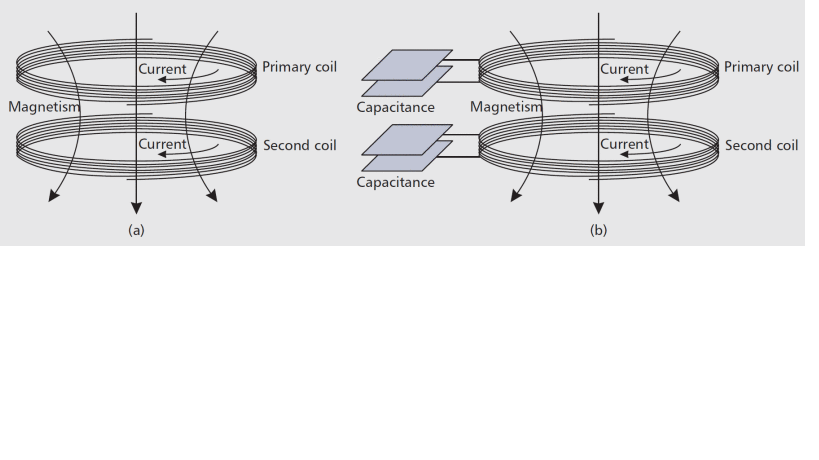
\includegraphics[scale=0.75]{Vildledning/Schematics/induktiv_resonans}
\caption{model af WPT setup \cite{mikro}}
\label{figure:wptsetup}
\end{figure}

Induktiv kobling. 
WPT ved induktiv kobling fungere, ved induktion over et magnetfelt mellem to spoler, hvilke genereres en strøm og spænding som ses på figur \ref{figure:wptsetup}a. Magnetisk induktiv kobling sker, når den primærspole som fungere som energi senderen genererer et vekselene magnetfelt på tværs af den sekundærspole, der er energien modtageren. Dette sker inden for et område generelt mindre end bølgelængden. Denne process skaber en near-field kraft, som induktiveres over den sekundære spole til en strøm/spænding, hvilket kan udnyttes af et trådløs apparatur, eksempelvis en mobil. \cite{mikro}
Fordelen ved induktiv kobling inkludere følgende; teknologien er nem, at implementer ved høj effektivitet, og det er sikkert for mennesker at være i nærheden af. Den er dog begrænset af afstand fra transmitter og receiver, idet at den har en effektiv energioverførelse mellem nogle få millimeter til et par centimeter. Ulemper ved induktiv kobling indebære den relative korte ladeafstand, varmen der udvikles i spolerne, og spolerne skal ligge meget tæt for, at kunne opnå den maksimale effekt.
Teknologien bliver i dag set i mobile enheder (mobiltelefoner og tablets), tandbørster, RFID-tags, induktionskomfur og betalingskort. \cite{mikro}

Resonant kobling. 
Magnetisk resonant kobling er baseret på kortvarige bølgekobling, hvilke genere og overføre en elektrisk strøm mellem to resonante spoler i et oscillerende eller varierende magnetfelt, som set på figur \ref{figure:wptsetup}b. Da de to spoler køre på samme resonant frekvens, kan der opnå en høj effektiv elektrisk energioverførelse, med meget lidt tab til  eksterne faktorer. Denne indskab gøre energioverførelsen næsten upåvirket af omgivelserne, hvilke også gør det muligt at lade selvom der er noget i mellem transmitter og receiver. 
Den klare fordel ved resonans kobling er den meget større effektive lade distance, som kan opnå en effekt på 90 procent optil 1 meter mellem transmitter og receiver, og 40 procent ud til to meter. \cite{mikro} Derudover kan en enkel transmitter lade flere receivere på samme tid så længe de operer på sammen resonans frekvens.
En af ulemperne ved resonant kobling er at hver receiver kræver en dedikeret kapacitets spole, hvilke gøre det svært at gøre receiveren lille nok til mobile enheder, og det gøre det generelt mere kompliceret at implementere. \cite{mikro}
\section{Faraday}
Fysikeren Michael Faraday beskrev, hvordan et skiftende magnetisk flux er i stand til at danne en elektrisk strøm. Den magnetiske flux angiver størrelsen på magnetfeltet i forhold til det givne areal, magnetfeltet påvirker. Den magnetiske flux afhænger af forskellige parametre, som spiller ind på at danne den elektriske strøm.

Den magnetiske flux er styret af arealet, den påvirker. Hvis størrelsen på det givne areal ændres, vil der også ske en ændring i den magnetiske flux. Hvis det gældende areal mindskes, vil den elektriske flux mindskes. Modsat vil en forøgelse af arealet medvirke, at den magnetiske flux øges.

\begin{figure}[H]
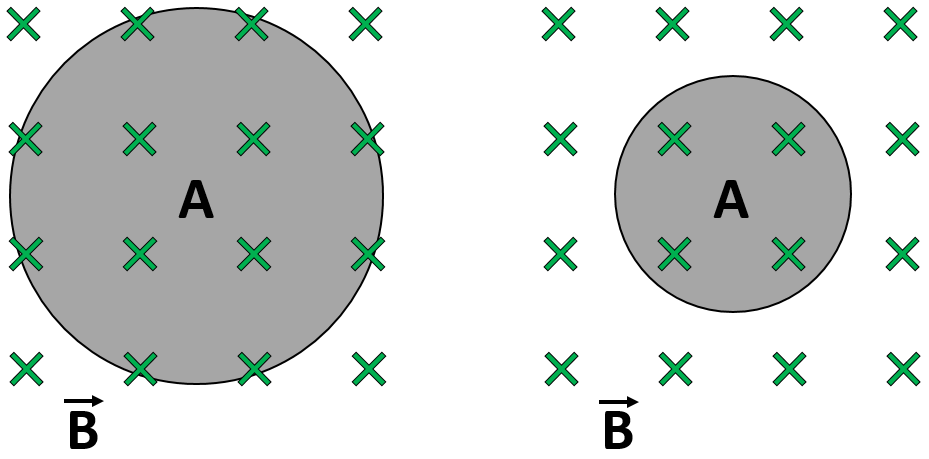
\includegraphics[scale=0.5]{Vildledning/Schematics/Areal_Bfelt}
\caption{Magnetfelt gennem arealet}
\end{figure}

Størrelsen på arealet, der bliver påvirket, er ikke kun afgjort af arealets dimentionen, men også vinklen for, hvordan den magnetiske feltlinjer står ind på det givne areal. Hvis feltlinjerne står vinkelret på det gældende areal, vil flest mulige feltlinjer ramme arealet. Hvis arealet står vinklet under $90^\circ$, vil nogle af feltlinjerne ikke løbe igennem og påvirke arealet, og den magnetiske flux mindskes. Er arealet parallelt med de magnetiske feltlinjer, så de få magnetiske feltlinjer som muligt påvirke arealet. Når vinklen ændres for de magnetiske feltlinjer og arealet, så vil den magnetiske flux også ændres.

\begin{figure}[H]
	\centering
	\begin{minipage}[b]{0.48\textwidth}
	\centering
	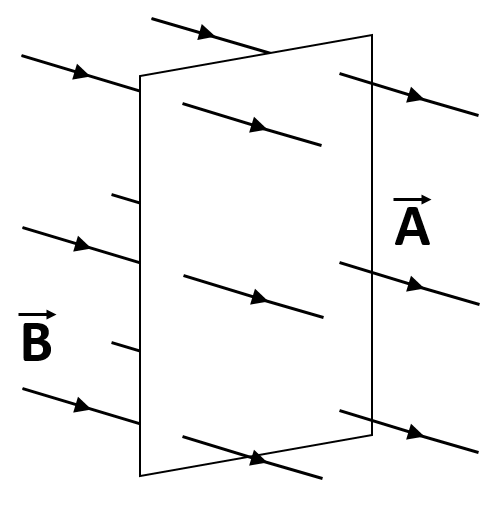
\includegraphics[width=0.5\textwidth]{Vildledning/Schematics/Magnetfelt_vinkelret} % Venstre billede
	\end{minipage}
	\hfill
	\begin{minipage}[b]{0.48\textwidth}
	\centering
	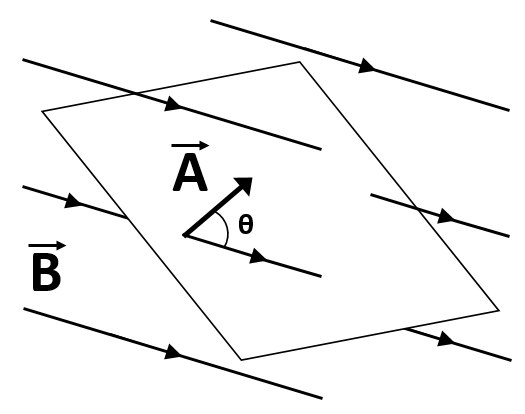
\includegraphics[width=0.5\textwidth]{Vildledning/Schematics/Magnetfelt_vinklet} % Højre billede
	\end{minipage}
\end{figure}

Størrelsen for de magnetiske feltlinjer er påvirket af strømstyrken for systemet. Ved en ændring af strømstyrken, vil de magnetiske feltlinjer ændre størrelse, hvorved den magnetiske flux vil varriere.
\section{Spoler's egenskaber}

En spole er en noget, der bliver brugt til mange forskellige ting, men det spolen bruges til er, at der sendes strøm igennem spolen, når strømen er blevet sendt igennem opstår der et magnetfelt omkring spolen. Magnetfeltet der bliver dannet omkring spolen, vil ligne det fra en magnet, men skal være af samme form så spolen. Feltet bliver meget kraftigere hvis der er jern inde i spolen. 

Hvis spolen kortsluttes mens der er strøm der løber igennem, vil spolen på bedst muligvis forsøge at opretholde strømmen, men da strømmen ikke kan løbe i en kreds kan det ikke lade sig gøre for spolen og opretholde strømmen.  Strømmen bruges i stedet i feltet, det vil sige at spændingen over spolens ender stiger voldsomt og der opstår ofte en gnist. Det er det samme der sker i tænd spolen i bilen eller i et køkken apparat eller lignende.

\begin{figure}[htbp]
	\centering
	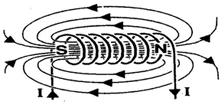
\includegraphics[width=0.5
	\textwidth]{Vildledning/Schematics/magnetfelt_omkring_en_spole.png}
	\caption{Magnetfelt omkring en spole.\cite{spoler}}
	\label{spole1}
\end{figure}

En magnet der er permanent, er også en metalgering, som der ofte er jern i, magneten får derved den egenskab, at den bliver magnetisk.  Bliver en permanent magnet skubbet over til noget der er kortsluttede, det kan være en spole sker der det, at den permanente magnet vil fremkalde strøm i spolen, når der er fremkaldt en strøm vil den permanente magnet forsøge, at holde feltet ude. Det betyder at spolen forsøger, at lave poler, som vil vende modsat af den permanente magnet. Men strømmen vil i løbet af meget kort tid forsvinde, hvis magneten ligger stille dette skyldes, at energien/strømmen vil blive omdannet til varme inde i spolens modstand. Hvis magneten derimod bliver fjernet sker der det omvendte, altså vil den påbegynde i det modsat retning, altså starte fra det felt der var inden magneten blev tilføjet. Ud fra dette kan det konkluderes, at der kun er strøm i spolen når der enten sættes et batteri til eller magnetfeltet ændres. Hvis feltet forbliver konstant vil strømmen forsvinde hurtigt og gå i nul dette skyldes også den ohmske modstand. 

En spole har ud fra dette altså ingen magnetfelt, medmindre den bliver påvirket af strøm, eller man påvirker den vedhjælp af magnetisme. 

Der findes en række stoffer ved lave temperaturer, disse stoffer er superledende, som også betyder, at de ingen elektrisk modstand har. Ingen elektrisk modstand betyder, at modstanden ligger på $0 \Omega$. Der er tale om legeringer af stoffer der er sjældne, men er almindelig kendte i blandt andet bly og kviksølv. Laves der en blyring, bly ringen bliver sat ved stuetemperatur hvor der bliver sat en permanent magnet igennem, hvis nu det hele bliver kølet ned til det absolutte nulpunkt som ca. er $-273^\circ C$, når dette er gjort fjernes den permanente magnet, når den permanente magnet er blevet fjernet, vil der ske det, som normalt sker ved induktion der vil nemlig opstå en strøm i blyringen, den strøm der opstår vil sørger for og genskabe det magnetfelt, som den permanente magnet havde. Der er ingen modstand hvilket også vil gøre, at strømmen vil forsætte, så der er et konstant magnetfelt, som magneten vil gå til det oprindelige magnetfelt. Magnetfeltet bliver målt i en enhed kaldet Tesla, som er opkaldt efter Nikola Tesla 1856-1943.\cite{spoler}


\input{limits} %% QI er inkluderet her %%
\section{Problemformulering}

\begin{itemize}

\item Hvordan kan resonant frekvens benyttes til at forbedre afstanden, hvor ved den trådløse opladning i en mobiloplader er effektiv.?

\end{itemize}


	\end{folderinput}
	
\begin{folderinput} {Teori}
\chapter{Teori}
\section{Reaktans til Impedans}
Reaktans:

Ved et LCR-kredsløb, så er der ikke kun tale om modstanden fra resistoren, men hvilken modstand kapacitoren og induktoren har. Den samlede modstand for kredsløbet kan beskrives igennem kompleks impedans, som er den samlede modstand for resistoren, kapacitoren og induktoren på kompleks form. Impedansen er essentiel til beskrivelse af den faseforskydelse, der kan opstå mellem spændingen og strømstyrken i LCR-kredsløbet.

For at forstå modstanden for en kapacitor og induktor, så skal begrebet reaktans bringes på banen. Ved elektriske felter er der tale om kapacitiv reaktans, som er gældende for kapacitorer, mens der for magnetiske felter er tale om induktiv reaktans, som er gældende for induktorer. Reaktansen for henholdsvis kapacitoren og induktoren er angivet, som deres modstand og optræder efter sammenhængen mellem strømstyrken og spændingen over kapacitoren og induktoren. Da de to komponenter ikke optræder ens i kredsløbet, er beregningerne for reaktansen forskellig. \cite{reaktans}

\begin{equation}
Kapacitiv reaktans: X_C = - \frac{1}{j \omega C}
\label{eq:kapacitivreaktans}
\end{equation}
\begin{equation}
Induktiv reaktans: X_L = j \omega L
\label{eq:induktivreaktans}
\end{equation}

I formel \ref{eq:kapacitivreaktans} og \ref{eq:induktivreaktans} indgår der to konstanter $C$ og $L$. C er en konstant for kapacitoren angivet som kapacitansen, mens $L$ er en konstant for induktoren angivet som induktansen. Omega beskrives som $\omega = 2 \pi f$, hvor $2 \pi$ svarer til én svingning, mens $f$ er frekvensen. $j$ angiver, at reaktansen er beskrevet som et kompleks tal.

Komplekse tal bliver benyttet for bedre, at kunne knytte spænding og strømstyrke sammen, så det kan afbilledes i forbindelse med den fastforskydelse, der kan forekomme. Dette forhold mellem spænding og strømstyrke kan udledes gennem omskrivning af sinus og cosinus, men for nemhedens skyld benyttes komplekse tal for at simplificere formlerne. Formlerne for reaktansen kan derved skrives om til: \cite{reaktans}

\begin{equation} 
Kapacitiv reaktans: X_C = - \frac{1}{j 2 \pi f C}
\end{equation}
\begin{equation}
Induktiv reaktans: X_L = j 2 \pi f L
\end{equation}

En perfekt kapasitor uden modstand ville forskyde bølgefunktionen for strømstyrken med $\frac{\pi}{2}$ frem for bølgefunktionen for spænding., hvilket svarer til en kvart svingning (1/4 frekvens). Modsat ville den perfekte induktor uden modstand sænke bølgefunktionen for strømstyrken med $\frac{\pi}{2}$ i forhold til bølgefunktionen for spænding.

Billeder af forskudte bølger (kapacitiv og induktiv reaktans)
\begin{figure}[H]
\centering
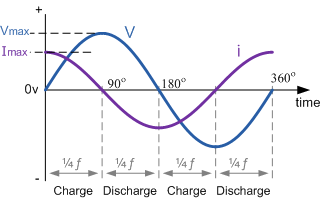
\includegraphics[scale=1.25]{Vildledning/Schematics/Kapacitiv_reaktans}
\caption{Kapacitiv reaktans \cite{kapasitans}}
\label{kreaktans}
\end{figure}
%Kilde: Capacitance in AC Circuit and Capacitive Reactance

\begin{figure}[H]
\centering
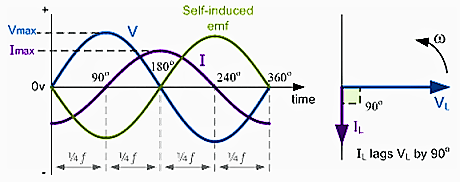
\includegraphics[scale=1.10]{Vildledning/Schematics/Induktiv_reaktans}
\caption{Induktiv reaktans \cite{kapasitans}}
\label{ireaktans}
\end{figure}
%Kilde: Inductive Reactance - Reactance of an Inductor

Da den komplekse impedans var LCR-kredsløbets samlede modstand, så kan det beregnes ved: \cite{impedans}
\begin{equation}
Z = R + j 2 \pi f L - \frac{1}{j 2 \pi f C}
\end{equation}
\newpage
\section{Magnetfelter og resonant frekvens}

Magnetisk induktiv kobling er i stand til at skabe en effektiv energioverførsel, hvor ca. 90 procent af den udsendte effekt bliver opfanget af modtageren. Dette kan samtidig gøres ved et lavt frekvensspektrum på 20 til 40kHz med en rækkevidde på op til 10cm. Magnetisk indukttiv kobling har en lille påvirkning på omkringliggende genstande, hvilket mindsker energispildet ved overførslen, men der er andre faktorer, der kan spille ind på, at effektiviteten for energioverførslen reduceres.

Placeringen for spolerne er ikke tilfældig, og det kan have en stor betydning for effektiviteten af energioverførslen, hvis spolerne ikke har direkte forbindelse. Det påvirker ikke magnetfelterne så meget, hvis paramagnetiske(ikke magnetisk) materiale er placeret mellem transistoren og modtageren. Magnetfelterne passerer gennem det paramegnetisk materiale, men bliver kun sænket af, at feltlinjerne magnetiserer partiklerne omkring. Til gengæld vil en forskydning af spolerne, eller at spolerne står vinklet på hinanden, reducere den optagede energi fra modtageren, da færre af de magnetiske feltlijner når modtageren.

\begin{figure}[H]
	\centering
	\begin{minipage}[b]{0.48\textwidth}
	\centering
	\includegraphics[width=0.5\textwidth]{Vildledning/Schematics/forskudt_spole} % Venstre billede
	\end{minipage}
	\hfill
	\begin{minipage}[b]{0.48\textwidth}
	\centering
	\includegraphics[width=0.5\textwidth]{Vildledning/Schematics/vinklet_spole} % Højre billede
	\end{minipage}
	\\ % Figurtekster og labels
	\begin{minipage}[t]{0.48\textwidth}
	\caption{Forskudte spoler} % Venstre figurtekst og label
	\label{fspoler}
	\end{minipage}
	\hfill
	\begin{minipage}[t]{0.48\textwidth}
	\caption{Vinklet spoler} % Højre figurtekst og label
	\label{vspoler}
	\end{minipage}
\end{figure}

Resonant frekvens:

Når der løber en strøm gennem et elektrisk kredsløb med vekselstrøm, så er der tilsvarende en frekvens for, hvor hurtigt strømmen skifter retning i systemet. Ved induktiv kobling er frekvensen med til at bestemme outputtet for det elektriske kredsløb. Den specifikke frekvens for et kredsløb, der giver det største output, kaldes for den resonante frekvens. For at energioverførslen mellem transistoren og modtageren skal være mest effektiv, så skal begge kredsløb have en ens resonant frekvens. Resonans frekvensen opretholdes ved en kapacitor koblet på transmitteren og receiveren. På denne måde bliver effekten udsendt med størst mulig output, og modtageren kan opfange effekten på bedst mulig vis.
\section{Faraday's lov}

Faraday's lov beskriver induktionen af elektricitet, ved hjælp af magnetisme. Herved omhandler det den magnetiske flux, i stedet for den elektriske flux, som bliver brugt ved Gauss's lov. Formlen for magnetisk flux er ens med formlen for den elektriske flux, dog hvor det elektriske felt er byttet ud med det magnetiske felt: $\Phi_B = \int \vec{B} \cdot \vec{dA}$

En induceret strøm opstår ikke fra den magnetiske flux alene, men ved en ændring i den magnetiske flux. Dette betyder, at der bliver induceret spænding, dvs. hvis der sker en ændring af magnetfeltets styrke, den påvirkede overflades størrelse eller vinklen for, hvordan det magnetiske felt går gennem den pågældende overflade.

Faraday benytter den magnetiske flux til, at beskrive den inducerede spænding ved \cite{fysikbog}:

\begin{equation} \label{faraday}
\centerline{$\varepsilon = -1 \cdot \frac{d \Phi_B}{dt}$}
\end{equation}

Ændringen af den magnetiske flux forekommer modsat af den inducerede spænding, så derfor ganges en faktor $-1$ på det differentierede udtryk af den magnetiske flux. Den magnetiske flux kan også beskrives som: $\vec{B} \cdot \vec{A}$ eller $B \cdot A \cdot cos(\theta)$.
\newpage
\end{folderinput}

	\begin{folderinput}{Lab}
\chapter{Forsøg}
\section{Antagelser forud for forsøg}

Forsøg med LC-kredsløb:

Spændingen over kapacitoren vil først stige og derefter falde, når frekvensen for systemet øges. Før den resonants frekvens opnåes vil spændingen stige langsomt. Nær den resonante frekvens vil der forekomme et udslag, hvor toppunktet for spændingen vil opstå. Efter toppunktet falder spændingen kraftigt, hvorefter faldet stilner af, så spændingen kun falder en smule ved stadig at øge frekvensen. Hvis den resonante frekvens ikke opnåes, så vil der ske en lille stigning i spændingsfaldet over kapacitoren.

Forsøg med LCR-kredsløb (Modstand):

Ved måling over modstanden i kredsløbet vil spændingen over modstanden stige i takt med frekvensen. Derved vil en øget frekvens tilsvarende resultere i et øget spændingsfald over modstanden.

Forsøg med LCR-kredsløb (Induktor):

Frekvensen er antal svingninger igennem systemet, og jo flere svingninger des større magnetfelt vil blive dannet ved induktoren. Spændingsfaldet over induktoren vil derved stige i takt med, at frekvensen stiger. Dette vil forekomme som en liniær rekretion, hvor frekvensen og spændingsfaldet stiger i takt med hinanden.
\section{Forsøg 1 - Kredsløb}

\subsection{Forsøgsbeskrivelse}

\subsubsection{Formål}
Formålet med disse forsøg er at for en forståelse af, hvordan de forskellige kredsløb fungere. Derudover bliver der også dannet en baggrundsviden af, hvordan det teoretiske er i kredsløbet. Måledataenes vær-dier kan senere bruges til, at beregne på de forskellige komponenter i kredsløbet. Ud fra måledataene kan der findes en induktans på spolen, som senere kan benyttes til værdi i Plecs, så vores forsøg beskrivelser også kan simuleres, derudover benyttes måledataene også til, at regne på andre forskellige komponenter. Alt dette findes i afsnittet med beregninger. Formlerne som bliver benyttet igennem dette afsnit, til at beregne på forsøget, er alle fundet i kilden \cite{fysikbog}.

\subsubsection{LC serie kredsløb}
%\textbf{LC Serie kredsløb}

Komponenter:

\begin{itemize}
\item Generator $(50\, \Omega$ modstand)
\item Kapacitor $( 0,1\, \mu F)$
\item Spole/Inductor $(1600$ vindinger)
\item Oscilloskop
\end{itemize}

Opstilling:

\begin{figure}[H]
\centering
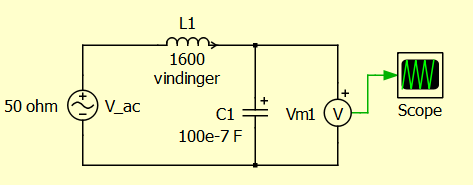
\includegraphics[scale=1]{Vildledning/Schematics/Kredslb/LC_Serie}
\caption{LC Serie Kredsløb}
\label{lcserie}
\end{figure}

Figur \ref{lcserie} viser, hvordan forsøgsopstillingen er bygget op. Forsøget består af en generator, spole og en kapacitor, hvor der sat et oscilloskop til.

\subsubsection{LC parallel kredsløb}

Komponenter:

\begin{itemize}
\item Generator $(600\, \Omega$ modstand)
\item Kapacitor $( 0,1\, \mu F)$
\item Spole/Inductor $(1600$ vindinger)
\item Oscilloskop
\end{itemize}

Opstilling:

\begin{figure}[H]
\centering
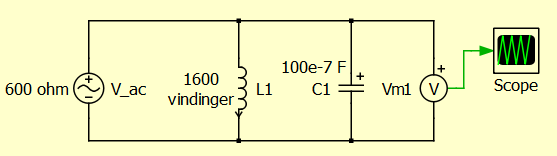
\includegraphics[scale=1]{Vildledning/Schematics/Kredslb/LC_Parallel}
\caption{LC Parallel Kredsløb}
\label{lcparallel}
\end{figure}

Figur \ref{lcparallel} viser forsøgsopstilling af et LC parallel kredsløb, hvor hele kredsløbet sidder parallelt. Kredsløbet er bestående af en generator, en spole og en kapacitor, hvor et oscilloskop er sat til.

\subsubsection{LCR målt over spolen}

Komponenter:

\begin{itemize}
\item Generator $(50\, \Omega$ modstand)
\item Kapacitor $( 0,1\, \mu F)$
\item Spole/Inductor $(1600$ vindinger)
\item Modstand/Resistance $(500\, \Omega)$
\item Oscilloskop
\end{itemize}

Opstilling:

\begin{figure}[H]
\centering
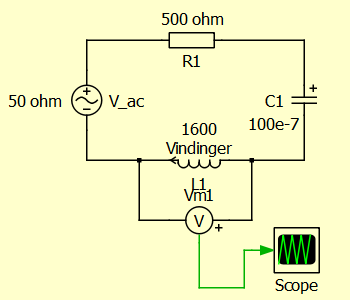
\includegraphics[scale=1]{Vildledning/Schematics/Kredslb/LCR_spole}
\caption{LCR-kredsløb målt over spolen}
\label{figure:lcrspole}
\end{figure}

Figur \ref{figure:lcrspole} viser forsøgsopstilling af et LCR-kredsløb. I dette forsøg bliver der målt over spolen, altså oscilloskopet er sat over spolen. Kredsløbet består af en generator, en spole, en kapacitor og en modstand.

\subsubsection{LCR målt over modstand}

Komponenter:

\begin{itemize}
\item Generator $(50\, \Omega$ modstand)
\item Kapacitor $( 0,1\, \mu F)$
\item Spole/Inductor $(1600$ vindinger)
\item Modstand/Resistance $(500\, \Omega)$
\item Oscilloskop
\end{itemize}


Opstilling:

\begin{figure}[H]
\centering
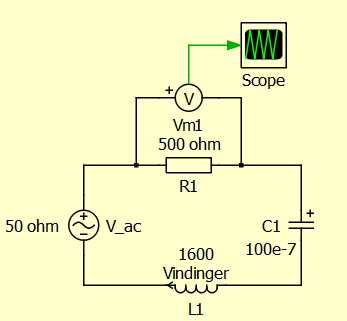
\includegraphics[scale=1]{Vildledning/Schematics/Kredslb/LCR_modstand}
\caption{LCR-kredsløb målt over spolen}
\label{lcrmodstand}
\end{figure}

Figur \ref{lcrmodstand} viser forsøgsopstilling af et LCR-kredsløb. Modsat tidligere forsøg, så bliver der målt over modstanden. Kredsløbet er bestående af samme komponenter som det tidligere forsøg.

\subsection{Fremgangsmåde}

Udførelsen af forsøgende er næsten ens, de variere ikke ret meget, forsøgsopstillingen bliver ændret fra forsøgs til forsøg, hvor der skiftets ud i komponenter, så det passer med det rigtige kredsløb.

Først opstilles kredsløbet, som det er vist på figurene \ref{lcserie}, \ref{lcparallel}, \ref{figure:lcrspole} og \ref{lcrmodstand}. Derefter skal oscilloskopet indstilles, så det måler de rigtige data, det indstilles til at måle en: peak-to-peak. Så er forsøget klar til at starte, der tændes for generatoren, og dens frekvens indstilles til den ønskede værdi, og peak-to-peak værdien noteres. Dette gøres med forskellige frekvenser, så der fås forskellige data, som senere kan plottes ind i en tabel, og der kan derved laves en graf for det.

\subsection{Resultater}

LC-kredsløb (Kapacitor):

For LC-kredsløbet blev der foretaget målinger for spændingen over kapacitoren ved forskellige frekvenser. Første måling er foretaget ved $1 \, kHz$, hvorefter de følgende målinger er foretaget med et $0,5\, kHz$ interval op til sidste måling ved $5,5\, kHz$. Resultaterne er indsat i nedenstående graf. Tabel \ref{tabular:lcserie} angiver resultaterne for spændingen i forhold til den givne frekvens.

\begin{figure}[H]
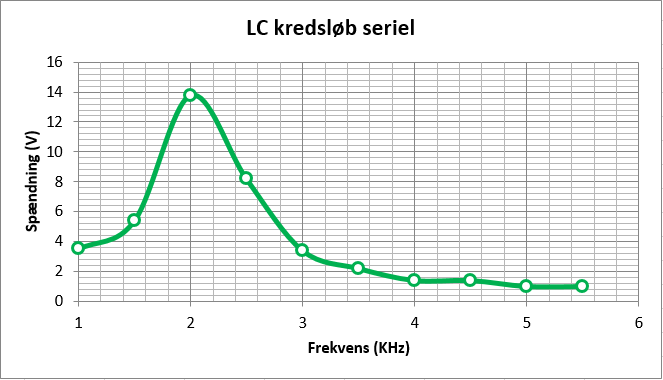
\includegraphics[scale=1]{Setup/Graf3}
\caption{}
\label{graph:lcserie}
\end{figure}

\begin{table}[H]
\centering
\begin{tabular}{|r|r|r|r|r|r|r|r|r|r|r|} \hline
kHz & 1 & 1,5 & 2 & 2,5 & 3 & 3,5 & 4 & 4,5 & 5 & 5,5 \\ \hline
V & 3,5 & 5,4 & 13,8 & 8,2 & 3,4 & 2,2 & 1,4 & 1,4 & 1 & 1 \\ \hline
\end{tabular}
\caption{}
\label{tabular:lcserie}
\end{table}

Graf \ref{graph:lcserie} viser sammenhængen mellem spændingen og frekvensen over kapacitoren, når frekvensen øges. Ved en frekvens på $1\, kHz$ er spændingen over kapacitoren $3,5\, V$. Ved en frekvens på $1,5\, kHz$ er spændingen øget til $5,4\, V$, hvorefter der sker en markant stigning til en spænding på $13,8\, V$ ved en frekvens på $2\, kHz$. Fra frekvensen på $2 kHz$ og til en frekvens på $4\, kHz$ er spændingen over kapacitoren faldet til $1,4\, V$, hvorefter funktionen flader ud, og spændingen næsten holdes stabil til en frekvens på $5,5\, kHz$.

LCR-kredsløb (Resistor):

Første sæt målinger for LCR-kredsløbet angiver spændingen over resistoren ved en stigende frekvens. Målingerne er foretaget fra $1\, kHz$ til $10\, kHz$ med et interval på $1\, kHz$ for hver måling. Resultaterne for målingerne er plottet i nedenstående graf. Tabel \ref{tabular:lcrmodstand} angiver resultaterne for spændingen i forhold til den givne frekvens.

\begin{figure}[H]
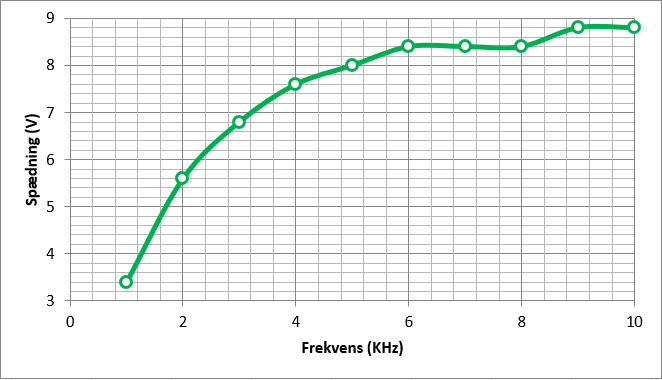
\includegraphics[scale=1]{Setup/Graf7}
\caption{}
\label{graph:lcrmodstand}
\end{figure}

\begin{table}[H]
\centering
\begin{tabular}{|r|r|r|r|r|r|r|r|r|r|r|} \hline
kHz & 1 & 2 & 3 & 4 & 5 & 6 & 7 & 8 & 9 & 10 \\ \hline
V & 3,4 & 5,6 & 6,8 & 7,6 & 8 & 8,4 & 8,4 & 8,4 & 8,8 & 8,8 \\ \hline
\end{tabular}
\caption{}
\label{tabular:lcrmodstand}
\end{table}

Graf \ref{graph:lcrmodstand} viser, hvordan spændingen over resistoren er lav ved en frekvens på $1\, kHz$. Ved en stigning i frekvens viser det sig, at spændingen følger en logaritmisk funktion, hvor den stiger meget i starten og begynder at flade mere ud, når frekvensen øges. Fra en frekvens på $1\, kHz$ til $4\, kHz$ stiger spændingen over modstanden fra $3,4\, V$ til $7,6\, V$, men ved de efterfølgende stigninger i frekvens flader funktionen ud, og der sker kun en spændingsstigning på $0,4\, V$ fra en frekvens på $6\, kHz$ til $10\, kHz$.

LCR-kredsløb (Spole):

De næste målinger der er foretaget på LCR-kredsløbet viser sammenhængen mellem spændingen og frekvensen for induktoren. Her foretages målingerne igen ved en frekvens fra $1\, kHz$ til $10\, kHz$ med et stigende interval på $1\, kHz$. Nedenstående graf viser resultaterne for forsøget, hvor tabel \ref{tabular:lcrspole} angiver resultaterne for spændingen i forhold til den givne frekvens.

\begin{figure}[H]
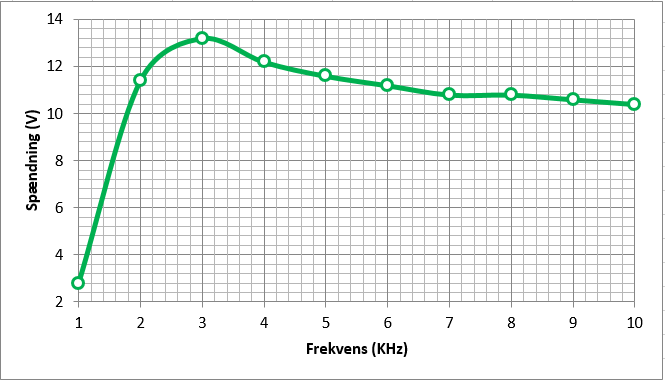
\includegraphics[scale=1]{Setup/Graf6}
\caption{}
\label{graph:lcrspole}
\end{figure}

\begin{table}[H]
\centering
\begin{tabular}{|r|r|r|r|r|r|r|r|r|r|r|} \hline
kHz & 1 & 2 & 3 & 4 & 5 & 6 & 7 & 8 & 9 & 10 \\ \hline
V & 2,8 & 11,4 & 13,2 & 12,2 & 11,6 & 11,2 & 10,8 & 10,8 & 10,6 & 10,4 \\ \hline
\end{tabular}
\caption{}
\label{tabular:lcrspole}
\end{table}

Spændingen over induktoren stiger fra $2,8\, V$ ved en frekvens på $1\, kHz$ til $11,4\, V$ ved en frekvens på $2\, kHz$. Spændingen stiger fortsat til $13,2\, V$ ved en frekvens på $3\, kHz$, hvorefter spændingen over induktoren begynder at falder ved en højere frekvens. Faldet i spændingen sker kun gradvist og ved en frekvens på $7\, kHz$, er funktionen næsten ved en stabil spænding.

\subsection{Databehandling}

%\subsubsection{"LC kredsløb"}

\begin{equation} \label{angfreq}
\omega = \frac{1}{\sqrt{LC}}
\end{equation}

Denne ligning for vinkelbestemt frekvens relaterer: frekvens, kapacitans og induktans.

Der løses for L da denne er besværlig at måle sammenlignet med den aflæste kapacitans. $\omega = 2\pi f$ så denne indsættes samtidigt:

\begin{equation}
\omega = \frac{1}{\sqrt{LC}} \Leftrightarrow L = \frac{1}{\omega^2 \cdot C} = \frac{1}{4\pi^2 f^2 \cdot C} = \frac{1}{4\cdot \pi^2 f^2\cdot 0.1\mu F}
\end{equation}


\subsubsection{LCR kredsløb}

\begin{table}[H]
\centering
\begin{tabular}{l|l}
Induktans  & 0,0525 $H$ \\ 
Kapacitans & 0.1 $\mu F$   \\
Amplitude  & 10,0 $V$   \\
Modstand   & 500 $\Omega$ \\
\end{tabular}
\caption{Værdier for komponenter}
\label{tabular:value}
\end{table}

I afsnit 4.2 blev der redegjort for resonant frekvens. Der blev nævnt at ved resonant frekvens, at strømmen gennem spolen og kapacitansen fuldstændig udeligner hinanden, altså strømmen gennem dem giver $0$.

Forsøget med LCR-kredsløbet afbillede, hvordan spændingen er afhængig af hvilken frekvens, der benyttes. Samtidig svinger den samlede impedans i kredsløbet og ud fra det, kan strømmen beregnes for kredsløbet. Ud fra dette viser det sig, at strømstyrken også varierer i forhold til frekvensen, hvor strømmen når maksimum ved systemets resonante frekvens. Her er modstanden afgørende for, hvordan strømstyrken opfører sig ved forskellige frekvenser. Ved en lav modstand i systemet vil strømstyrken ved den resonante frekvens være meget høj i forhold til andre frekvenser, mens en stor modstand vil mindske udslaget. Til gengæld vil en stor modstand forstørre frekvensområdet, som strømstyrken vil toppe ved.

\begin{figure}[H]
\centering
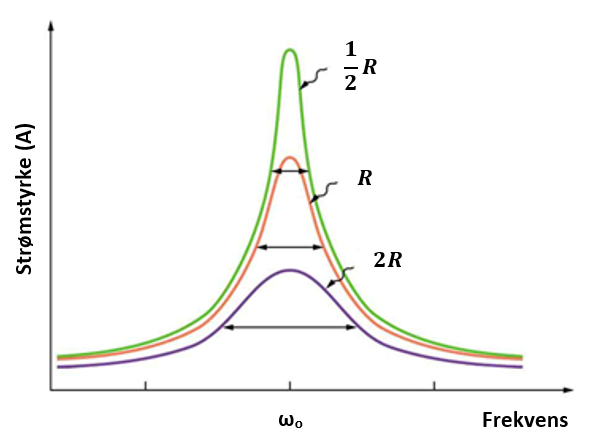
\includegraphics[scale=0.75]{Vildledning/Schematics/Resonanskurver}
\caption{Resonant frekvens ved 3 forskellige modstande \cite{Bresonant}.}
\label{figure:resonantfrekvens}
\end{figure}

Graf \ref{figure:resonantfrekvens} viser tre forskellige grafer over strømstyrken for systemet i forhols til frekvensen. Forskellen på de tre funktioner er, at der er forskellige størrelse modstande til de tre kredsløb. Den grønne graf har en modstand på $\frac{1}{2} R$, hvor strømstyrken giver et stort udsving ved den resonante frekvens. Til gengæld er udsvinget meget smalt, så frekvensen skal ikke afvige meget fra den resonante frekvens, før strømstyrken falder kraftigt. Ved den orange funktion er modstanden i systemet fordoblet. Her foretager strømstyrken igen et stort udsving ved den resonante frekvens, men stadig mindre end den grønne funktion. Til gengæld er udsvinget fladet mere ud, hvorved der kan ske større afvigelser fra den resonante frekvens, uden strømstyrken falder meget. For den lilla funktion, hvor modstanden er på $2 R$, så er udsvinget for strømstyrken lav ved den resonante frekvens i forhold til de to andre funktioner. Derimod strækker grafens udsving sig over et stort frekvensområde.

Grafen viser, at den resonante frekvens vil være optimal for det største output. Herefter afbilleder funktionerne, at den samlede modstand for systemet er afgørende for, hvor stort et output systemet har, og hvor let det er at ramme et højt output. Hvis der skal benyttes en lav strømstyrke, vil det være optimalt at benytte en stor modstand i kredsløbet for at give et bredt frekvensspektrum til den ønskede strøm. Derimod kræver høje output, at modstanden er lavt, hvorved der opstår et stort udslag, men så skal der omhyggeligt korrigeres for den resonante frekvens.

Resonant frekvens er givet ved:

\begin{equation} 
\omega_0 = \frac{1}{\sqrt{LC}}
\label{eq:resonant}
\end{equation}

Med $\omega_0 = 2 \pi f$, dvs. at $\omega_0$ er lig med en fuld svingning $(2\pi)$ ganget med frekvensen $(f)$. Så kan ligning \ref{eq:resonant} løses for frekvensen $f$.

\begin{equation} 
\omega_0 = \frac{1}{\sqrt{LC}} \Leftrightarrow f = \frac{1}{2 \cdot \sqrt{C \cdot L} \cdot \pi}
\label{eq:resonantfrekvens}
\end{equation}

Værdierne fra tabel \ref{tabular:value} benyttes i formlen \ref{eq:resonantfrekvens}, og så findes den resonante frekvens for LCR-kredsløbet.

\begin{equation*}
f = \frac{1}{2 \cdot \pi \cdot \sqrt{(0,1 \cdot 10^-6 F) \cdot 0,0525 H}} = \underline{2197 \, Hz}
\end{equation*}

I afsnit 4.1 og (Impedans afsnit) er der blevet redegjort for formlen for Impedans, den bliver defineret som, $Z$, hvor $Z = R + (X_L - X_C)$. $X_L$ og $X_C$ er blevet nævnt i \vref{eq:kapacitivreaktans} og\vref{eq:induktivreaktans}. Formlen for Impedans bruges også i formlen for at finde peak på strøm igennem kredsløbet. Formlen for strøm peak er:

\begin{equation} 
I_p = \frac{V_p}{\sqrt{R^2 + (X_L - X_C )^2}} = \frac{V_p}{Z}
\label{eq:peak}
\end{equation}

Hvor $V_p$ er volt peak for kredsløbet, denne findes ved: $V_p = \sqrt{V^2_{Rp} + (V_{Lp} - V_{Cp})^2}$, og Impedansen er givet ved $Z = \sqrt{R^2 + (X_L - X_C)^2}$. Så kan de kendte værdier indsættes, og der kan opstilles en graf for $I_p$ og frekvens $f$. Alle data findes i Bilag B (Label til bilag b). Der laves udregninger for en frekvens på $2000 \, Hz$.

$2000 \, Hz$:

$V_p$, $X_L$ og $X_C$ beregnes ud fra formlerne nævnt tidligere.

\begin{equation*}
X_L = 2\pi \cdot 2000 \, Hz \, \cdot 0.0525 \, Hz \, = 659,734 \Omega
\end{equation*}

\begin{equation*}
X_C = \frac{1}{2\pi \cdot 2000 \, Hz \, \cdot (0.1 \cdot 10^{-6} \, F)} = 795,775 \Omega
\end{equation*}

\begin{equation*}
V_p = \sqrt{(9,3 \, V)^2 + (12,3 \, V - 14,8 \, V)^2} = 9,63 V
\end{equation*}

Så kan strøm-peak $I_p$ beregnes:

\begin{equation*}
I_p = \frac{9,63 \, Hz}{\sqrt{(500 \Omega)^2 + (659,734\Omega-795,775\Omega)^2}} = 0,01858 A \cdot 1000 = \underline{18,58 \, mA}
\end{equation*}

Derved er strøm-peak udregnet med en frekvens på $2000 \, Hz$. Denne fremgangsmåde benyttes til at udregne for alle frekvenser, altså fra $1000 \, Hz$ til $10000 \, Hz$, disse data findes i Bilag B (Label dertil). Datasættene er ikke resultaterne fra forsøgene, men de er aflæst efter simulationer af kredsløbet opsat i Plecs. Simulationerne har samme værdier for komponenterne, som komponenterne benyttet i forsøgsopstillingerne.

Ud fra målingerne over LCR-kredsløbet kan strømstyrken for systemet beregnes ud fra en given frekvens, som foretaget tidligere. Herefter kan beregningerne verificeres ved at holdes op mod angivne data fra en simulation af samme kredsløb.

Resultaterne fra simulationen kan også benyttes til at vise udviklingen for strømstyrken ved ændring af frekvensen. Derudover kan der ændres på størrelsen for modstanden på resistoren i systemet for at se, hvordan strømstyrken ændre sit udsving omkring den resonante frekvens.

\begin{figure}[H]
\centering
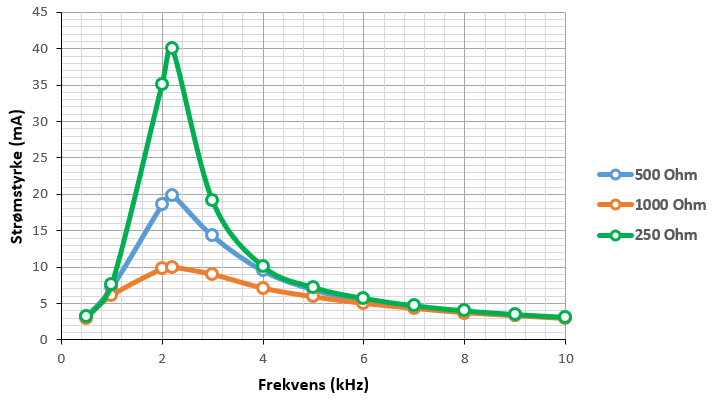
\includegraphics[scale=0.75]{Vildledning/Schematics/Graf_forsg1}
\caption{}
\label{figure:forsg1}
\end{figure}

Graf \ref{figure:forsg1} viser tre funktioner for strømstyrken ved en stigende frekvens. Forskellen på de tre sæt data for funktionerne er, at de henholdsvis har indsat en modstand på $250 \Omega$, $500 \Omega$ eller $1000 \Omega$. Funktionen med modstanden på $250 \Omega$ giver et stort udslag i løbet af en stigning i frekvens mellem $1 kHz$ og $2 kHz$. Toppunktet for funktionen er skarpt optegnet ved den resonante frekvens, hvorefter strømstyrken er blevet mere end halveret ved en frekvens på $3 kHz$. På højere frekvenser falder strømstyrken fortsat, men faldet stilner roligt af. Ved funktionen med en modstand på $500 \Omega$ er udsvinget for strømstyrken ved den resonante frekvens halveret i forhold til første funktion. Til gengæld sker faldet ved større frekvenser ikke så drastisk. Derved bliver frekvensspektret forstørret for et fornuftigt strømstyrkeoutput. Ved den sidste funktion med en modstand på $1000 \Omega$ er udslaget ved den resonante frekvens næste jævnet ud sammenlignet med de to andre funktion. Til gengæld er faldet for strømstyrken lille, og frekvensområdet for en stabil strømstyrke er forlænget meget i forhold til de første to funktioner. Sammenlignet med funktionen med $250 \Omega$, er det overordnede fald i strømstyrken lav for funktionen med $1000 \Omega$ modstand. Funktionen med en modstand på $250 \Omega$ falder med op til 75 procent i strømstyrke fra den resonante frekvens på $2,197 kHz$ til en frekvens på $4 kHz$, hvorimod funktionen med en modstand på $1000 \Omega$ kun falder med 30 procent i strømstyrke over samme frekvensområde.

\subsubsection{Beregning af den elektromotoriske spænding}

Ved induktiv kobling er det muligt at beregne den inducerede elektromotoriske spnæding ved hjælp af den magnetiske flux. Ifølge Faraday's lov er den elektromotoriske spænding beskrevet som det negative differentiale af den magnetiske flux i forhold til tiden.

Den benyttede induktor i forsøget er en cylinderformet spole. Det magnetiske felt for spolen er angivet som $\mu_o \cdot n \cdot I$, hvor n er antal vindinger for spolen, og I er strømstyrken. For at beregne den samlede magnetiske flux dannet i spolen, så skal arealet for den cylinderformede spoles tværsnit og længden for spolen ganges på. Tværsnitsarealet for spolen kan opskrives som $2 \pi r^2$, så den magnetiske flux kan beregnes ved $\Phi_B = \mu_o \cdot n \cdot I \cdot 2 \cdot \pi \cdot r^2 \cdot l$. Induktansen for spolen beregnes ved $\mu_o \cdot n \cdot 2 \cdot \pi \cdot r^2$, hvilket kun består af konstanter, så den magnetiske flux kan beskrives som $\Phi_B = L \cdot I$.

Den elektromotoriske spænding for spolen kan nu beskrives ved Faraday's lov:

\begin{equation}
\xi = - \frac{d\Phi_B}{dt}
\end{equation}

Herved kan udtrykket for den magnetiske flux indsættes, så den elektromotoriske spænding kan beregnes ved:

\begin{equation}
\xi = - L \cdot \frac{dI}{dt}
\end{equation}

Faraday's lov beskrives her, hvordan størrelsen på den elektromotoriske spænding er afhængig af en varierende strømstyrke. Strømstyrken kan beskrives ved $I_o \cdot sin(\omega \cdot t + \varphi$, hvor $I_o$ er amplituden for sinusfunktionen, omega er $2 \cdot \pi \cdot f$ og $varphi$ angiver faseforskydelsen for funktionen.

Ved forsøget med LCR-kredsløbet, hvor der foretages målinger over spolen, er det største udslag for spændingen ved $3 kHz$ med en spænding på $13,2 V$. Ved systemet er der indsat en modstand på $500 \Omega$, så amplituden kan beregnes ved $I_o = \frac{U}{R} = \frac{13,2 V}{500 \Omega} = 26,4 mA$. Strømstyrken kan herefter beskrives som en funktion af tiden ved:

\begin{equation}
I = 26,4 mA \cdot sin(2 \pi \cdot 3 kHz \cdot t + \varphi)
\end{equation}

Faseforskydelsen $\varphi$ varierer mellem 0 og $\frac{\phi}{2}$. Hvis forkydelsen er 0, følger funktionen for strømstyrken og spændingen hinanden. Hvis faseforskydelsen er på $\frac{\phi}{2}$, vil funktionen følge en cosinus i stedet.

Herfra kan udtrykket for strømstyrken indsættes i formlen for den elektromotoriske spænding, som derved bliver:

\begin{equation}
\begin{aligned}
&\xi = - L \cdot \frac{dI}{dt} = - 42,3 mH \cdot 26,4 mA \cdot cos(2 \pi \cdot 3 kHz \cdot t +\varphi) \cdot 2 \pi \cdot 3 kHz \\
&= cos(18,85 kHz \cdot t + \varphi) \cdot 21,05 H \cdot A \cdot Hz
\end{aligned}
\end{equation}

Da der ingen tid $(t)$ er, så kan denne ikke beregnes. Ved en kendt tid er det muligt at beregne den elektromotoriske spænding ved modtagerspolen. Beregningen tager udgangspunkt i at finde den overførte energi fra transmitteren til modtageren. Faraday's lov kan benyttes til at beregne det teoretiske udbytte af elektromotorisk spænding ved modtageren ved omdannelse af den magnetiske flux afsendt fra transmitteren. Det skal dog siges, at beregningerne går ud fra, at hele magnetfeltet fra transmitteren når ud til modtageren, så intet går tabt til omgivelserne i luften. Derfor skal resultatet for den elektromotoriske spænding ganges med nyttivirkningen (Se forsøg 2).

Ud fra forsøgende med LCR-kredsløb kom der forskellige værdier for strømstyrken, hvor der tydeligt sker ændringer, afhængig af frekvensen. Ved den resonante frekvens $(2197 \, Hz)$ sker der en stor ændring i strøm, hvor den når helt op på $20,00 \, mA$, hvor den på mindre frekvenser er væsentligt lavere. Ved højere værdier på modstanden sker der også en ændring i værdien for resonant frekvens, højere modstand er lig lavere resonant frekvens, som videre giver en lavere effekt $(mA)$.

\newpage

\section{Forsøg 2 - IKEA-oplader} \label{sec:forsg2}

I dette forsøg undersøges sammenhængen mellem afstanden af oplader: senderen og telefonen: modtageren med henblik på tabet af energi når der sker en trådløs opladning, og afstanden mellem sender og modtager vokser. Altså effektiviteten $\eta$ undersøges ved forskellige afstande mellem sender og modtager.

\subsection{Forsøgsbeskrivelse} 
\subsubsection{Komponenter}

\begin{table}[htbp] %% Komponenter tabel %%
\begin{tabular}{l|l|c|l}
        & Strømforsyning               & Oplader             & Cover               \\ \hline
Model:  & KMW-190-330-GS               & MORIK, E1404        & VITAHULT, 22974     \\
Input:  & 220-240V$\sim$50/60Hz, 0.18A & 19V$\sim$1.74A, 33W & 5 W       \\	
Output: & 19V$\sim$1.74A, 10W          & 5W                  & 5V, 1A             
\end{tabular}
\caption{Alt er aflæst direkte fra komponenternes etiketter.}
\label{table:sender}
\end{table}

%%%%%%%%%%%%%

\begin{table}[htbp]
\begin{tabular}{l|lcl}
         & Iphone 4 &          &        \\ \hline
Batteri: & Li-Po     & 1420 mAh & 5,3 Wh
\end{tabular}
\caption{Aflæst fra \cite{batteri}}
\label{table:batteri}
\end{table}

Strømkilden til strømforsyningen er et standart ikke jordet, tobenet, europæisk væg stikkontakt, 230 volt 50 Hz.

Som modtager er der benyttet en \textbf{Iphone 4}, \textit{Model A1332 EMC 380A med FCC ID: BCG-E2380A, IC: 579C-E2380A.}\footnote{Aflæst fra bagsiden af enheden.}
Denne enhed er udstyret med cover, model og egenskaber kan ses i tabel \ref{table:sender}. Her er det dog vigtigt at notere sig at telefonen er brugt, og er en ældre model (købt november 2011). Altså er batteriet ikke i fabriksny tilstand. Det er usikkert om dette har haft en relevant effekt på det udførte forsøg. Da dette kan have en effekt på hvordan batteriet lader. I forsøget er der antaget at opladningen sker lineært, mere om dette i følgende sektioner.

Ydermere er der benyttet papir til at lægge imellem mobilen med coveret og opladeren for at øge afstanden mellem dem, så det magnetiske felt forstyrres mindst muligt, og afstanden er holdt fast. 

\begin{figure}
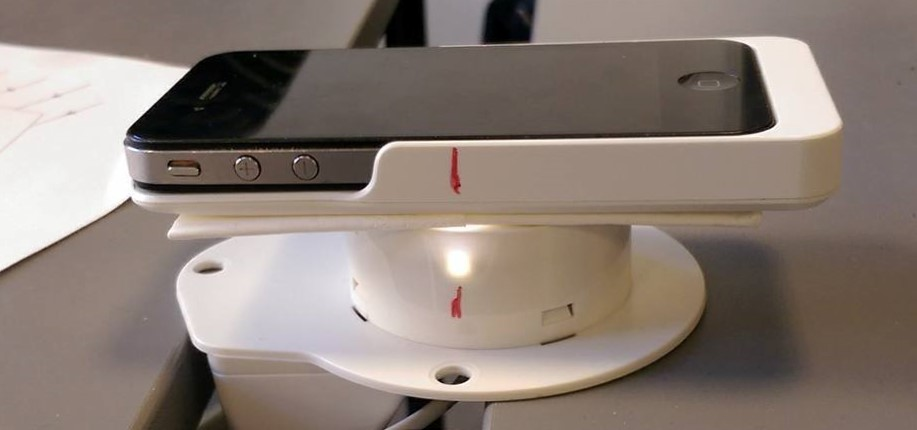
\includegraphics[width=1\textwidth]{Vildledning/Schematics/forsg2_opstilling1}
\caption{Opstilling med Iphone 4 og IKEA oplader L = 0,25 cm}
\label{figure:opstilling}
\end{figure}

\subsubsection{Fremgangsmåde}

Udførelsen af forsøget er meget simpel, og består af to dele der gentages tre gange. Første del er at bestemme hvor højt modtager telefonen skal være løftet fra opladeren. Altså længden L bestemmes i cm, hvor positiv retning er væk fra opladeren. Anden del er at aflæse telefonens batteriprocent hvert tiende minut. Dette gentages med tre forskellige værdier for L, altså tre forskellige afstande.

Alle tre gange sikres der at koblingen ikke er ustabil. Hjælp til at opnå dette er en diode, i opladeren, der lyser konstant hvis koblingen er stabil. For at opnå denne stabile kobling placeres telefonen midt ovenpå opladeren, så spolerne i henholdsvis sender og modtager ligger direkte ovenpå hinanden. Hertil er der tegnet en rød streg på både oplader og cover, det det er muligt at afgøre at coveret ligger samme sted under hvert forsøg.

Første L værdi er valgt til 0 cm da dette teoretisk set burde være den optimale kobling mellem sender og modtager i et system designet til trådløs energioverførsel. Det ses også i den første graf der hvor $L = 0$ at denne opnår den højeste ladningsprocent. Det skal dog noteres at spolerne i sender og modtager ikke lægger præcist direkte ovenpå hinanden da der er et lag plastik og et gummikryds imellem. Disse antages ikke at have nogen effekt på opladningen. Længden L starter fra den hvide plastikskive med gummikrydset på opladeren, altså direkte ovenpå. Den præcise afstand mellem plastic og spole i senderen er ukendt. Det samme gælder i coverets ydre plastiklag, hvor dennes tykkelse og afstand mellem den og modtager spolen også er ukendt.

Tiden er målt hvert tiende minut (bilag \ref{bilag:forsg2}) og målt med en afvigelse på $\pm 5$ sekunder, hvilket burde være hurtigt nok til ikke at se en ændring i ladningsprocenten.

Til slut undersøges værdien af L hvor der ikke er muligt at danne en kobling, altså der hvor dioden stopper med at lyse og der ikke sker en opladning af batteriet.

\subsubsection{Resultater}
Det ses at op til omkring L = 1 cm, at det ikke er muligt at danne en forbindelse mellem opladeren og coveret med telefonen i.

Rå, ikke redigeret, data kan ses i bilag \ref{bilag:forsg2}. Disse data er benyttet til at opstille de følgende tre diagrammer:

\begin{figure}[H]
\centering
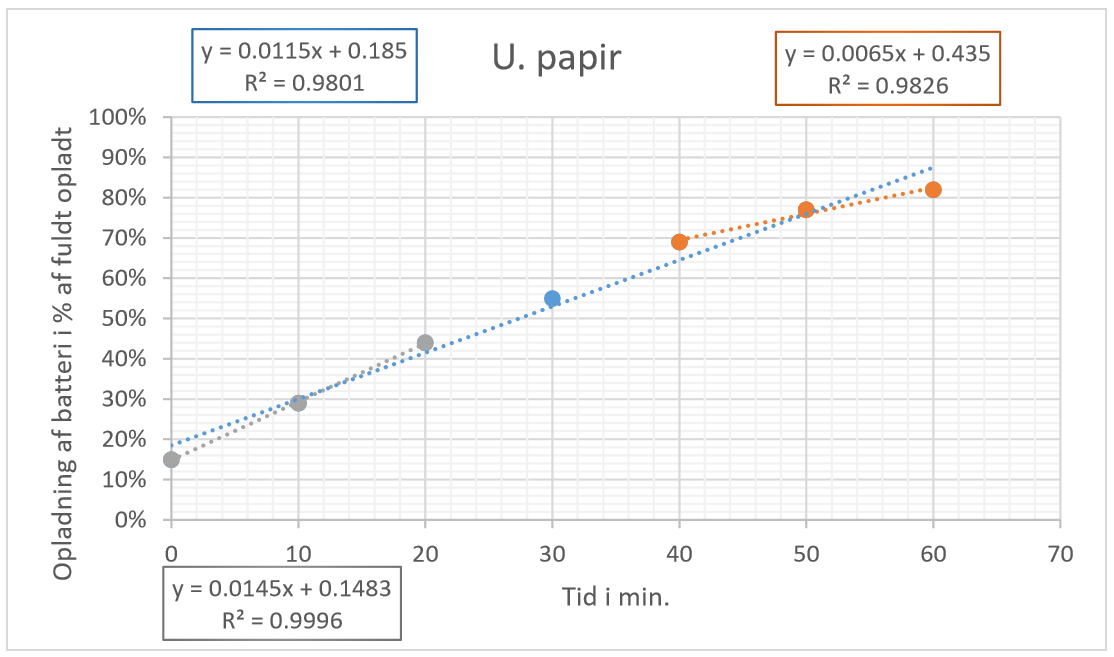
\includegraphics[width=1\textwidth]{Setup/forsg2_graf1}
\caption{}
\label{figure:graf1}
\end{figure}

\begin{figure}[H]
\centering
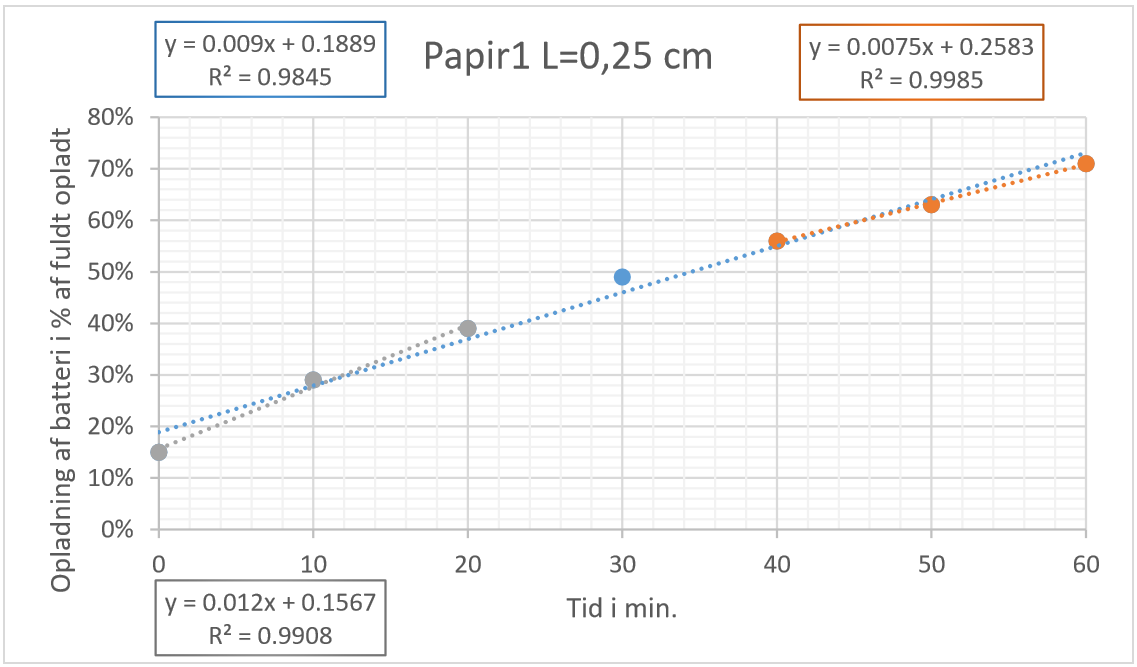
\includegraphics[width=1\textwidth]{Setup/forsg2_graf22}
\caption{}
\label{figure:graf2}
\end{figure}

\begin{figure}[H]
\centering
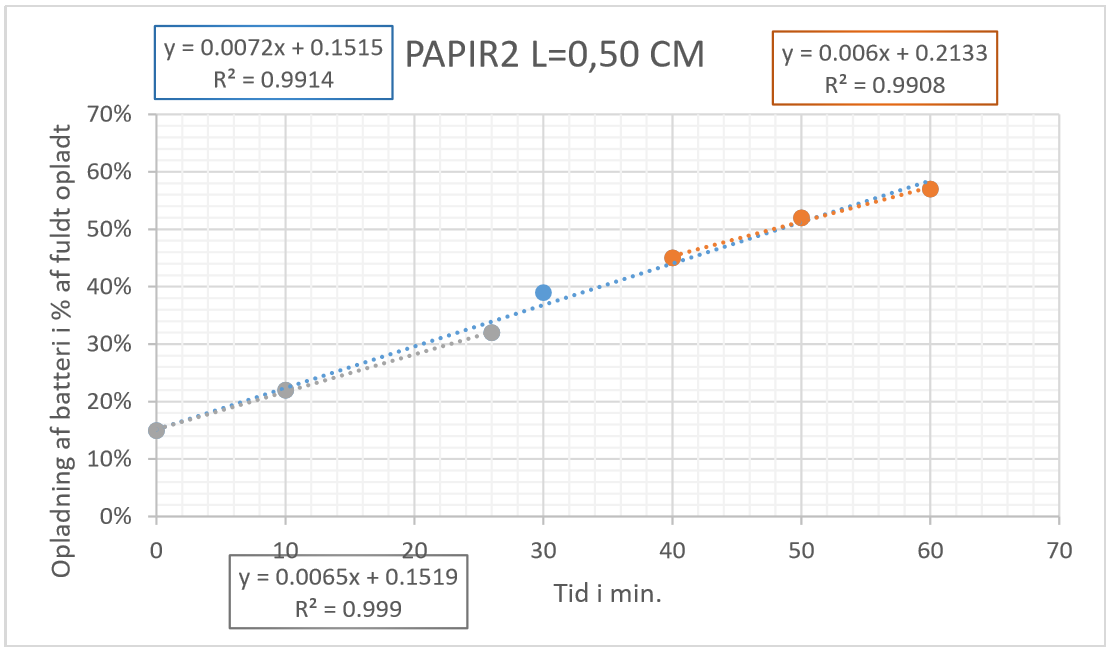
\includegraphics[width=1\textwidth]{Setup/forsg2_graf3}
\caption{}
\label{figure:graf3}
\end{figure}

I første forsøg hvor $L = 0$ ses det at opladning af batteriet nåede op på 82 procent ladning af maksimal ladning på batteriet (100 procent), indenfor den målte tidsperiode på 60 minutter. I de to næste forsøg ender opladningsprocenten efter 60 minutter på henholdsvis 81 procent og 57 procent ved $L = 0.25$ og $L = 0.5$ aflæst fra datasættet i bilag \ref{bilag:forsg2} og ses tydeligt på figur \ref{figure:graf1}, figur \ref{figure:graf2} og figur \ref{figure:graf3}.

Der er lavet tre lineære regressioner per diagram, en af de tre førstedatapunkter en for de tre sidste og den over dem alle samlet. Her ses det at opladningen ikke sker helt lineært, altså at opladningen sker ved samme hastighed gennem hele forløbet. Ved sammenligning af hældningskoefficienten af de tre første punkter og tre sidste punkter ses det at opladningen er mere effektiv i starten af opladningen end den er til slut f.eks. i figur \ref{figure:graf1} hvor $0,012\, \frac{E_\%}{t} > 0,009\, \frac{E_\%}{t}$.

Den ikke lineære opladning kan skyldes af et væld af ting, hvor det er antaget at det ikke er skyldt af den trådløse opladning, men snarere faktorer som: et ældre batteri, smartchargin teknologi\footnote{Det er ikke undersøgt om den målte telefon har disse teknologier eller hvordan de fungerer, på højere end basis niveau.} eller andet software der har en effekt på batteriet el. andet. 

\subsection{Databehandling}
I denne sektion undersøges det, ud fra det begrænsede datasæt, hvor stor effektivitet der mistes ved at forlænge afstanden mellem oplader og telefon med cover. Dette undersøges ved at beregne forskellige nyttevirkninger for den varierende værdi af L. 

Det antages at når batteriets batteri procent kan aflæses til 100 \% på telefonens display at batteriet indeholder $O_{maks}=1432\, mAh \approx 5,3 Wh$. Dette benyttes så til at udregne nyttevirkningen $\eta$ med watt time værdier.

Det aflæses i skemaet \ref{table:sender} at opladeren har en effekt på 5 W og coveret har en en effekt på $(5 V \cdot 1 A = 5 W)$. Hvis det antages at der bliver ladt op telefonens batteri med den fulde mulige effekt gennem hele forsøget (lineær opladning) kan der bestemmes hvilken procent batteriet skulle kunne aflæses til efter 60 minutter:

\begin{equation}
O_{maks60}= \frac{5 W\cdot 1h}{5,3Wh} \cdot 100 \approx 94 \%
\label{eq:omaks}
\end{equation}

Dette er så den teoretiske maksimale opladningsprocent batteriet kan ende på. Denne viser også hvor meget der kan lades på batteriet på 60 minutter:
\begin{equation}
\Delta O_{maks} = 5 W \cdot 1 h = 5Wh
\end{equation}

Altså er den maksimale mængde watt timer den givne oplader kan påføre batteriet 5. I alle forsøgene starter mobilen på 15 \% opladning af de 5,3 Wh så:
\begin{align*}
O_{start} = 5,3 \cdot 0,15 = 0,8 Wh
\end{align*}
 

\textbf{1. kør}

I det første forsøg ender telefonen på 82 \% efter 60 minutter så:
\begin{align*}
& \Delta O_{1\%} = 82\%-15\% =  67\%  \\
& \Delta O_1 = 5,3 Wh \cdot 0,67 = 3,6 Wh
\end{align*}


Nyttevirkningen (i \%) kan nu beregnes vha. $\Delta O_1$ og $\Delta O_{maks}$:  
\begin{equation}
\eta_1 = \frac{\Delta O_1}{\Delta O_{maks}} \cdot 100 = \frac{3,6 Wh}{5 Wh} \cdot 100 \approx 86 \%
\label{eq:nyt1}
\end{equation}

Dette gøres ved de to næste forsøg, stadig efter 60 minutters opladning.

\textbf{2. kør:}
\begin{align*}
& \Delta O_{2\%} = 71\%-15\% =  56\%  \\
& \Delta O_2 = 5,3 Wh \cdot 0,56 = 3 Wh
\end{align*}
Nyttevirkningen beregnes:
\begin{equation}
\eta_2 = \frac{\Delta O_2}{\Delta O_{maks}} \cdot 100 = \frac{3 Wh}{5 Wh} \cdot 100 = 60 \%
\label{eq:nyt2}
\end{equation}

\textbf{3. kør:}
\begin{align*}
& \Delta O_{3\%} = 57\%-15\% =  42\%  \\
& \Delta O_3 = 5,3 Wh \cdot 0,42 = 2,2 Wh
\end{align*}
Nyttevirkningen beregnes:
\begin{equation}
\eta_3 = \frac{\Delta O_3}{\Delta O_{maks}} \cdot 100 = \frac{2,2 Wh}{5 Wh} \cdot 100 \approx 44 \%
\label{eq:nyt3}
\end{equation}

De tre værdier for $\eta$ stilles op i et $(L,\eta)$ koordinatsystem ser det således ud som i figur \ref{figure:graf4}

\begin{figure}[H]
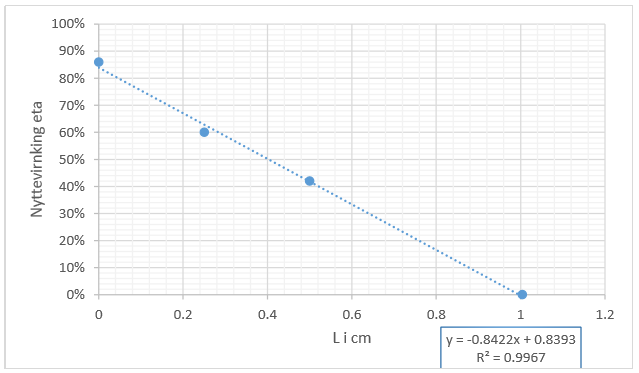
\includegraphics[width=1\textwidth]{Setup/forsg2_graf4}
\caption{}
\label{figure:graf4}
\end{figure}
I samme omgang laves der en lineær regression men kun af de tre målte punkter, dette aflæses til:
\begin{equation}
y=-0,8422x+0,8393 \Rightarrow \eta = -0,8422L+0,8393
\label{eq:regression}
\end{equation}
Det sidste punkt der er skæringen med x-aksen bestemmes ud fra regressionen \ref{eq:regression}:
\begin{align*}
& solve(\eta =-0.8422L+0.8393,L) \\
& \Leftrightarrow L = 1,003964 \approx 1 cm
\end{align*} 
Dette er så den maksimale værdi for L, altså den maksimale afstand mellem opladerens overflade og telefonen med cover. Dette virker som en brugbar projektion da det er tæt på den maksimale L værdi som der blev målt til under forsøget, der var lige under 1 cm. Dette vil så sige at den bestemte lineære ligning til en vis grænse kan benyttes til at vise en sammenhæng mellem afstanden og nyttevirkningen, og i sidste ende hvor meget power man kan få ud af opladeren. I hvert fald for den givne IKEA oplader.

Altså i de tre forsøg formåede den trådløse oplader fra IKEA at overføre 3,6 Wh, 3,0 Wh og 2,2 Wh som henholdsvis er en nyttevirkning på 86 \%, 60 \% og 44 \% for de tre fors. Altå er det tydeligt at når afstanden L mellem sender og modtager vokser mindskes energioverførslen betydeligt. Ud fra de tre forsøg og den dannede prognose ses det at den benyttede IKEA (QI) opladers nyttevirkning ændrer sig ud fra ligning \ref{eq:regression}.
	\end{folderinput}

%	\begin{folderinput}{Beregninger}
%\chapter{Forsøgsberegninger}

\begin{itemize}
\item \textcolor{red}{Her kommer der til at være en intro til hvad vi vil have ud af beregningerne.}
\end{itemize}

\section{LC kreds}

\begin{equation} \label{angfreq}
	\omega = \frac{1}{\sqrt{LC}}
\end{equation}

Denne ligning for vinkelbestemt frekvens relaterer: frekvens, kapacitans og induktans.

Der løses for L da denne er besværlig at måle sammenlignet med den aflæste kapacitans. $\omega = 2\pi f$ så denne indsættes samtidigt:

\begin{equation}
	\omega = \frac{1}{\sqrt{LC}} \Leftrightarrow L = \frac{1}{\omega^2 \cdot C} = \frac{1}{4\pi^2 f^2 \cdot C} = \frac{1}{4\cdot \pi^2 f^2\cdot 0.1\mu H}
\end{equation}

\begin{itemize}
\item \textcolor{red}{frekvensens her skulle nok være resonant frekvens $\omega_0$ for kredsløbet, denne er vi nød til at finde først måske ved hjælp af $I_p$ s. 615}
\end{itemize}
%	\end{folderinput}

%	\begin{folderinput}{Vildledning}
%\chapter{Forsøg 1} \label{bilag:forsg1}

P1 - Gruppe C-16a - 07-Nov-16

\begin{figure}[htbp]
\centering
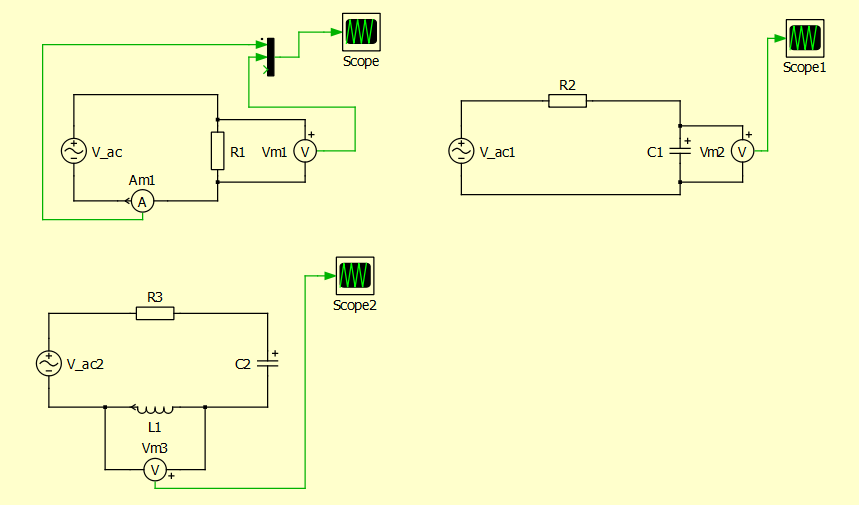
\includegraphics[width=1\textwidth]{Vildledning/Schematics/Eks1_LCR.png}
\caption{Foreslåede eksperiment kredsløb. R-kreds - CR-kreds - LCR-kreds}
\label{fig:Eks1}
\end{figure}
\newpage

\section{Hvad vil vi opstille?}
\begin{itemize}
\item R-kreds
\item CR-kreds
\item LCR-kreds
\end{itemize}
Til alle opstillingerne vil der i starten benyttes et oscilloskop som kilde, sat til vekselspænding ved 5 V, 50Hz.

De tre opsætninger benyttes som reference punkter til videre eksperimentring.  
\section{R-kreds}
Til at starte med vil vi opstille, det måske aller simpleste kredsløb, ved bare at sende en vekselspænding over en resistor og måle spændingsforskellen og strømmen over det.

Herefter vha. $U=R\cdot I$ kan der så undersøges om den aflæste værdi af resistoren er den samme som den målte.
\section{CR-kreds}
Opstillingen her er ens med R-kredsen, uden ampere-meter, bare at der nu er sat en kapacitator på og volt-meteret er flyttet hen over kapacitatoren.

Herefter ses der på om der er sket en ændring i spændingsforskellen over kapacitatoren, sammenlignet med den mængde spænding der er tilført systemet.
\section{LCR-kreds}
Dette er den vigtigste kreds der undersøges, da der nu er lavet et loop ved at sætte en spole i kredsløbet. Volt-meteret der benyttes her skulle gerne være et der kan tegne grafer, specifikt $(U,t)$.

Kredsløbet er en forlængelse af de to andre. Volt-meteret er nu bare flyttet til hen over spolen, da dette er den komponent med størst relevans.

Her undersøges der den spændingskurve der kan tegnes over spolen. Denne kan herefter sammenlignes med kurven i givet fra en simulering i Plecs. Dette er selvfølgelig kun relevant hvis det er muligt at komme tæt på virkelige værdier i programmet.

%	\end{folderinput}
	
	
\bibliography{bib/bibfil} %% Litteraturlisten indsættes her %%


\appendix
\clearforchapter
\phantomsection
\pdfbookmark[0]{Appendiks}{appendiks}
\chapter{Forsøg 1} \label{bilag:forsg1}

P1 - Gruppe C-16a - 07-Nov-16

\begin{figure}[htbp]
\centering
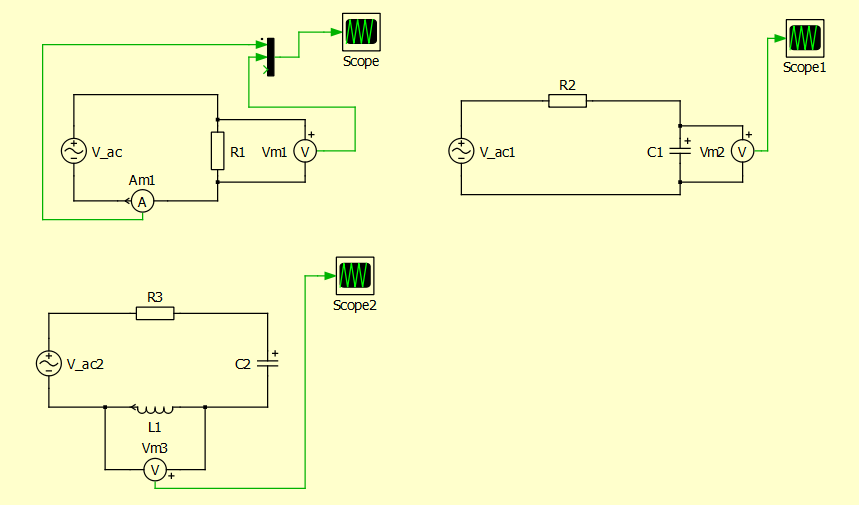
\includegraphics[width=1\textwidth]{Vildledning/Schematics/Eks1_LCR.png}
\caption{Foreslåede eksperiment kredsløb. R-kreds - CR-kreds - LCR-kreds}
\label{fig:Eks1}
\end{figure}
\newpage

\section{Hvad vil vi opstille?}
\begin{itemize}
\item R-kreds
\item CR-kreds
\item LCR-kreds
\end{itemize}
Til alle opstillingerne vil der i starten benyttes et oscilloskop som kilde, sat til vekselspænding ved 5 V, 50Hz.

De tre opsætninger benyttes som reference punkter til videre eksperimentring.  
\section{R-kreds}
Til at starte med vil vi opstille, det måske aller simpleste kredsløb, ved bare at sende en vekselspænding over en resistor og måle spændingsforskellen og strømmen over det.

Herefter vha. $U=R\cdot I$ kan der så undersøges om den aflæste værdi af resistoren er den samme som den målte.
\section{CR-kreds}
Opstillingen her er ens med R-kredsen, uden ampere-meter, bare at der nu er sat en kapacitator på og volt-meteret er flyttet hen over kapacitatoren.

Herefter ses der på om der er sket en ændring i spændingsforskellen over kapacitatoren, sammenlignet med den mængde spænding der er tilført systemet.
\section{LCR-kreds}
Dette er den vigtigste kreds der undersøges, da der nu er lavet et loop ved at sætte en spole i kredsløbet. Volt-meteret der benyttes her skulle gerne være et der kan tegne grafer, specifikt $(U,t)$.

Kredsløbet er en forlængelse af de to andre. Volt-meteret er nu bare flyttet til hen over spolen, da dette er den komponent med størst relevans.

Her undersøges der den spændingskurve der kan tegnes over spolen. Denne kan herefter sammenlignes med kurven i givet fra en simulering i Plecs. Dette er selvfølgelig kun relevant hvis det er muligt at komme tæt på virkelige værdier i programmet.

\chapter{Forsøg 2} \label{bilag:forsg2}

\begin{figure}[htbp]

\centering
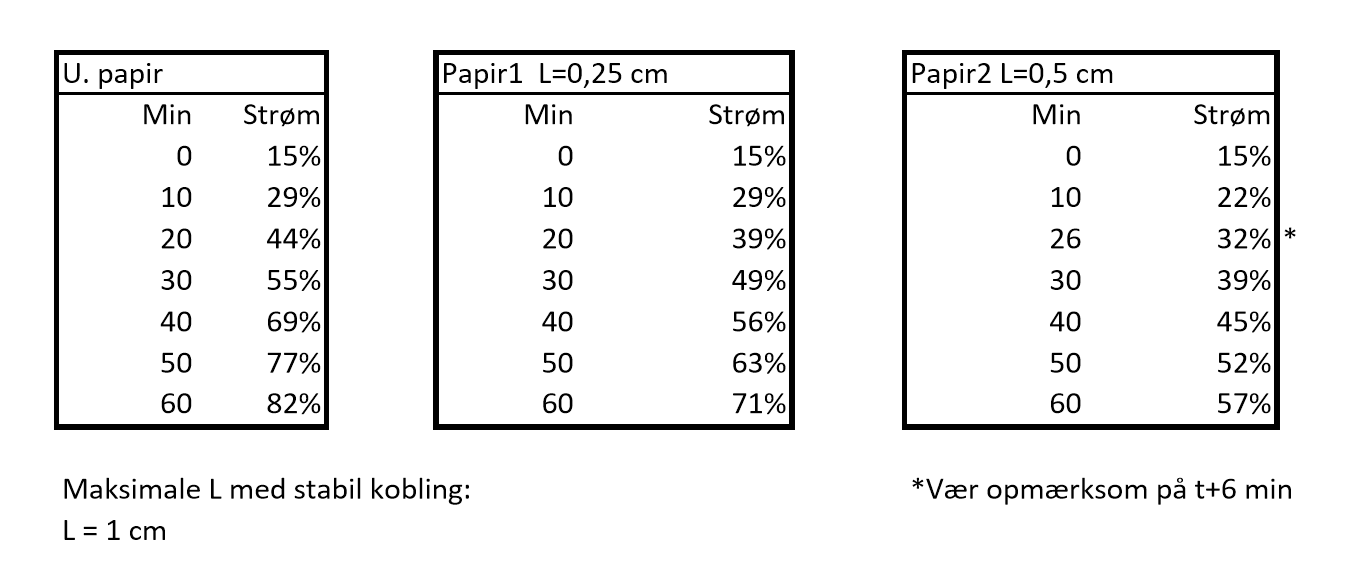
\includegraphics[width=1\textwidth]{Setup/forsg_2_bilag2}
\label{figure:forsg2}

\end{figure}

%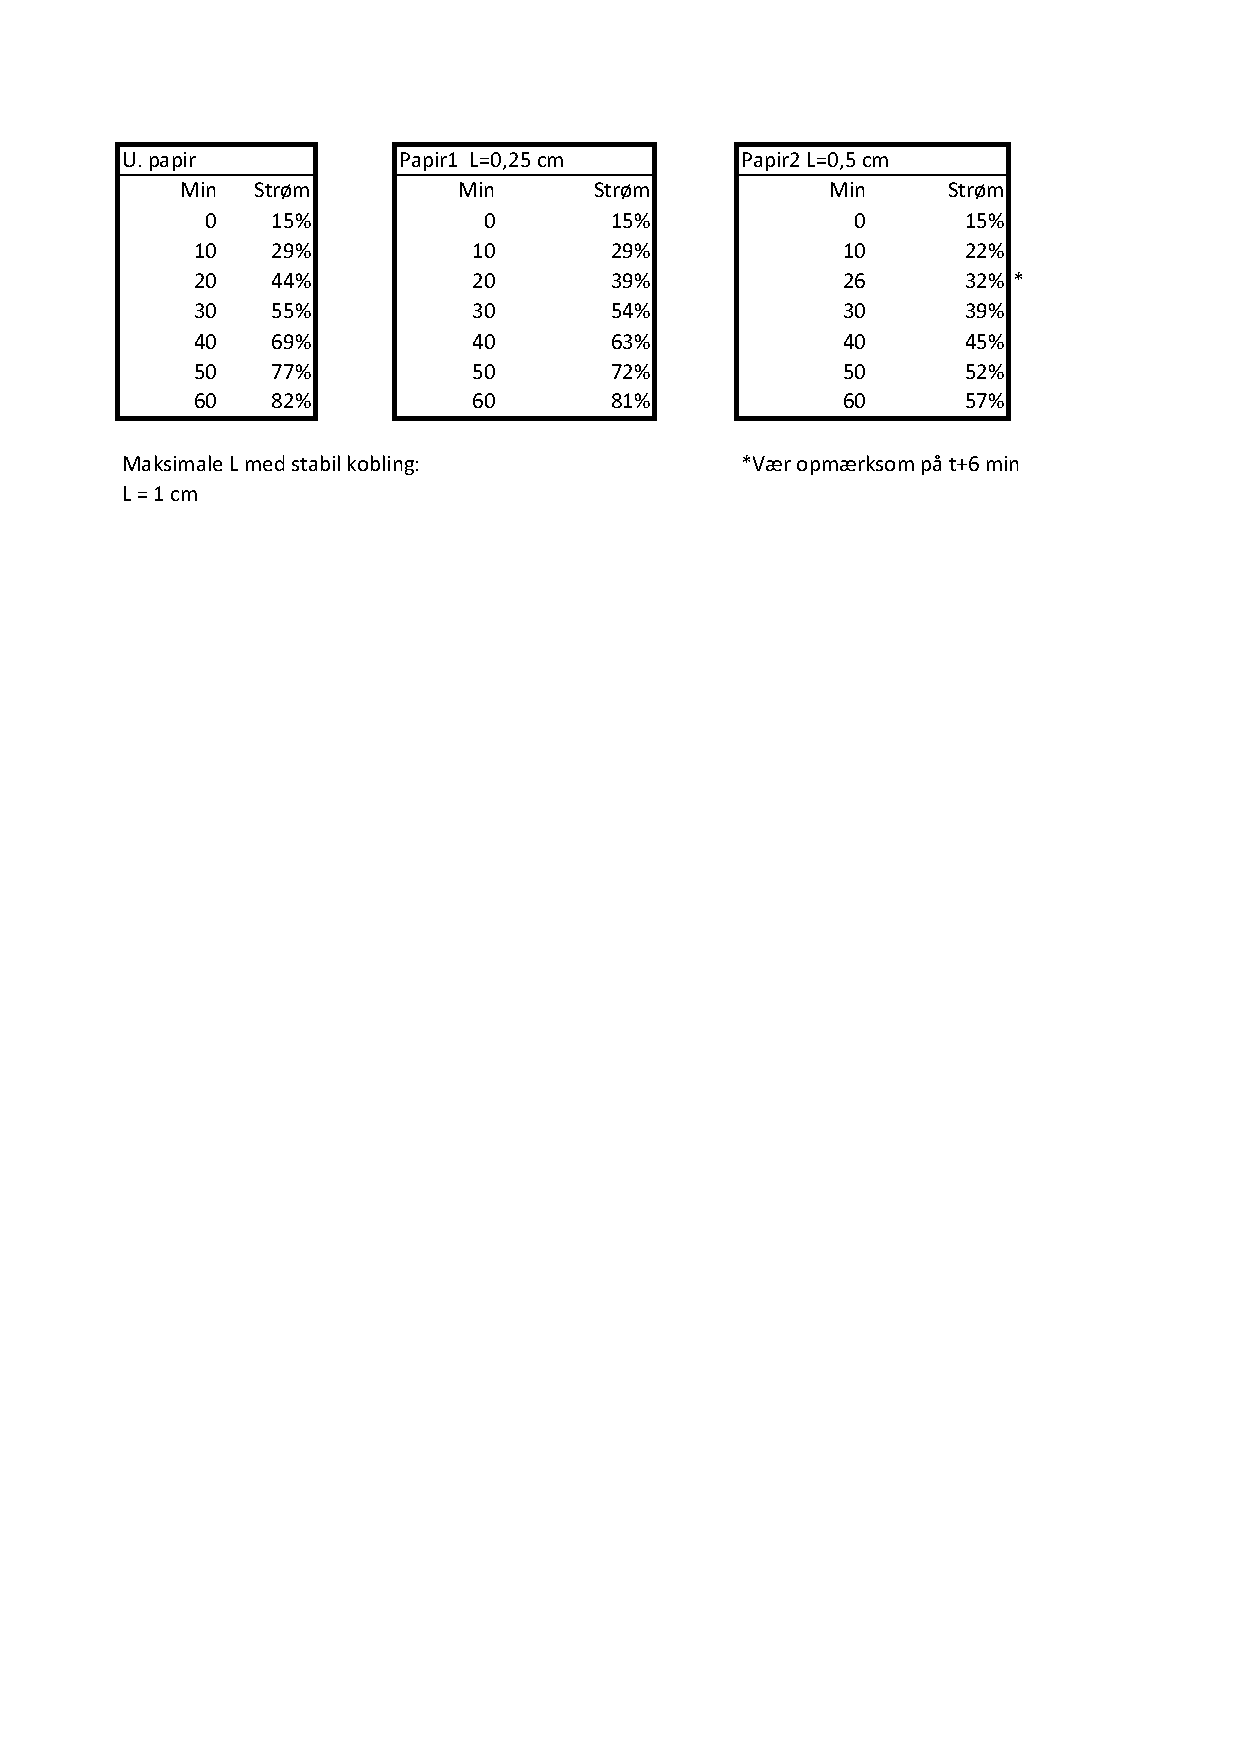
\includepdf[pages={1}]{Setup/forsg_2_bilag.pdf} Includere en pdf af bilaget

%\chapter{PV-fremadrettet}
Nu da vi har lavet vores første forsøg, hvor vi har set på, hvordan spændingen skifter over en modstand, kapacitator og spole ved ændring på frekvensen, kan vi nu gå videre til vores forsøg om WPT. Vi fik chancen for at omlægge den teori, vi har læst om, ud til en forsøgsopstilling, hvor vi kunne aflæse forskellige resultater, der giver mulighed for videre arbejde. Det har ikke lokket os fra at skulle arbejde videre med projektet, snarere det modsatte. Vi har fået nyt blod på tanden og glæder os til de afsluttende forsøg. Forsøgene skal benyttes til databehandlingen, så vi kan sammenligne resultaterne, så vi har konkrete tal at arbejde ud fra, når vi skal videre med problemløsningen. Vores strategi for fremtiden er at vi vil skriftes til at lave forsøg og dobbelttjekke hinandens forsøgsopstillinger. Når den ene del af gruppen er i laboratorierne vil den anden del af gruppen ihærdigt skriver videre, laver beregninger, skematics osv. til rapporten. Det er vores målsætning at holde møde hver fredag, så vi kan holde trit med vores tidsplan, og at hvis vi kommer bag ud, er det muligt for de andre i gruppen at træde til og hjælpe et medlem. Dette er ingen individuel rapport, og vi skal alle sammen kunne stå inde for rapporten. Ergo er det vigtigt, at man hjælper hinanden, for hvis der er en som taber, taber hele gruppen. Det er lige meget hvis skyld, det er, for vi er alle i samme båd.

For at holde gejsten oppe i gruppen sørger vi for at holde hinanden i nakken, så der ikke er nogen, der får problemer og falder bagud i forhold til gruppen. Projektet er en samlet indsats, så det er vigtigt at få lavet opsamlinger i gruppen, så alle kan følge med, og alle har samme udgangspunkt for senere arbejde. Derudover diskuterer vi om, hvad der interesserer os ved projektet, og hvad vi gerne vil have ud af det færdige produkt, så det holder os fast på et endeligt mål. Hvis vi arbejder med det, vi finder interesse for, er det lettere at holde sig fokuseret på arbejdsopgaverne, og man får lyst til at gøre en god indsats (ikke kun for en selv, men også for gruppen som helhed).

Som gruppe bliver vi enige om, hvilke arbejdsområder vi skal undersøge og skrive om. Herefter inddeler vi os i mindre grupper for hver arbejdsopgave (2-3 mand pr. gruppe). Dette gør, at vi hurtigt kan få indsamlet brugbar viden og udført en stort stykke arbejde, men at vi samtidig ikke står alene med en opgave. Det at være i små grupper gør også, at man kan få flere input og idéer til, hvad man eventuelt kan bringe ind over opgaven, hvilket gør at projektet bliver mere nuanceret. For at holde styr på, hvor langt hver gruppe er, og hvad de hver især har skrevet, så holder vi jævnligt møder til at opsummere processen.

Da vi er igennem problemanalysen, så har vi fået dannet os en god grundviden om projektet, som vi videre kan benytte til forsøg, modeller og projektløsningen senere hen. Dette betyder også, at vi nu skal til at specificere os på enkelte dele af projektet, så vi får indsnævret vores undersøgelser.

\end{document}